 %%%%%%%%%%%%%%%%%%%%%%%%%%%%%%%%%%%%%%%%
% Stylish Article
% LaTeX Template
% Version 2.1 (1/10/15)
%
% This template has been downloaded from:
% http://www.LaTeXTemplates.com
%
% Original author:
% Mathias Legrand (legrand.mathias@gmail.com) 
% With extensive modifications by:
% Vel (vel@latextemplates.com)

% License:
% CC BY-NC-SA 3.0 (http://creativecommons.org/licenses/by-nc-sa/3.0/)
%
%%%%%%%%%%%%%%%%%%%%%%%%%%%%%%%%%%%%%%%%%
%----------------------------------------------------------------------------------------
%	PACKAGES AND OTHER DOCUMENT CONFIGURATIONS
%----------------------------------------------------------------------------------------

\documentclass[10pt]{SelfArx} % Document font size and equations flushed left
%encoding
\usepackage{geometry}
 \geometry{
 a4paper,
 total={170mm,257mm},
 left=6mm,
 right=6mm,
 top=0mm,
 bottom=10mm
 }
 \usepackage{tikz,pgfplots}
\usepackage{lmodern}
\usepackage{indentfirst}
\usepackage{booktabs}
\usepackage{scrextend}
\changefontsizes[11pt]{10pt}

%OPCAO PARA POR DENTRO DOS PARENTESIS 
% SelfArx

%--------------------------------------
\usepackage[utf8]{inputenc}
\usepackage[T1]{fontenc}
\usepackage{gensymb}
\usepackage{amsmath}
%\usepackage{multirow}
\usepackage{caption}
%-------------------------

%\usepackage[english]{babel} % Specify a different language here - english by default
\usepackage[portuguese]{babel}
%Hyphenation rules
%--------------------------------------
\usepackage{hyphenat}
\hyphenation{mate-mática recu-perar}
%-------------------------------------

\usepackage{lipsum} % Required to insert dummy text. To be removed otherwise

%----------------------------------------------------------------------------------------
%	COLUMNS
%----------------------------------------------------------------------------------------

%\setlength{\columnsep}{0.55cm} % Distance between the two columns of text
\setlength{\fboxrule}{0.0pt} % Width of the border around the abstract

%----------------------------------------------------------------------------------------
%	COLORS
%----------------------------------------------------------------------------------------

\definecolor{color1}{RGB}{0,0,0} % Color of the article title and sections
\definecolor{color2}{RGB}{0,50,150} % Color of the boxes behind the abstract and headings

%----------------------------------------------------------------------------------------
%	HYPERLINKS
%----------------------------------------------------------------------------------------

\usepackage{hyperref} % Required for hyperlinks
\hypersetup{hidelinks,colorlinks,breaklinks=true,urlcolor=color2,citecolor=color1,linkcolor=color1,bookmarksopen=false,pdftitle={Title},pdfauthor={Author}}

%----------------------------------------------------------------------------------------
%	ARTICLE INFORMATION
%----------------------------------------------------------------------------------------

\JournalInfo{Instituto Superior Técnico} % Journal information
\Archive{MEFT 2019/2020 \\ Oscilações e Ondas \\ Junho de 2020} % Additional notes (e.g. copyright, DOI, review/research article)

\PaperTitle{\begin{center}O Bongo de Feynmann\end{center}} % Article title
\Authors{\begin{center} Thomas Gaehtgens \textit{ist186809}
\end{center}} % Authors


\Keywords{} % Keywords - if you don't want any simply remove all the text between the curly brackets
\newcommand{\keywordname}{} % Defines the keywords heading name

%----------------------------------------------------------------------------------------
%	ABSTRACT
%----------------------------------------------------------------------------------------
\Abstract{Pretende-se com este trabalho simular os modos de vibração do bongo onde Feynmann tocava, acompanhado pelo seu amigo, Ralpha Leighton, temas célebres com \textit{orange juice}. Para tal, aproximou-se a membrana do instrumento de percussão a uma membrana circular e simulou-se o sistema em \textit{Python}.} 
%\comment{ Ralph Leighton é o amigo do Feynmann que alinha nas batucadas rs rs rs
%----------------------------------------------------------------------------------------

\begin{document}

\flushbottom % Makes all text pages the same height

\maketitle % Print the title and abstract box

%\tableofcontents % Print the contents section

\thispagestyle{empty} % Removes page numbering from the first pages

%----------------------------------------------------------------------------------------
%	ARTICLE CONTENTS
%----------------------------------------------------------------------------------------

\section*{Suposições Físicas} % The bitch of a \section*{} command stops section numbering 

Antes de se deduzir o problema da membrana de raio a, impuseram-se as algumas características ao sistema para facilitar o estudo do mesmo. \par A massa da membrana por unidade de área é constante, a tensão por unidade de comprimento devido ao estiramento da membrana é constante em todos os pontos e direções, não mudando durante o movimento e por fim, o deslocamento da membrana é pequeno em relação ao tamanho da membrana.

\vspace{-0.3cm}
\begin{figure}[ht]
\centering
\captionsetup{justification=centering}
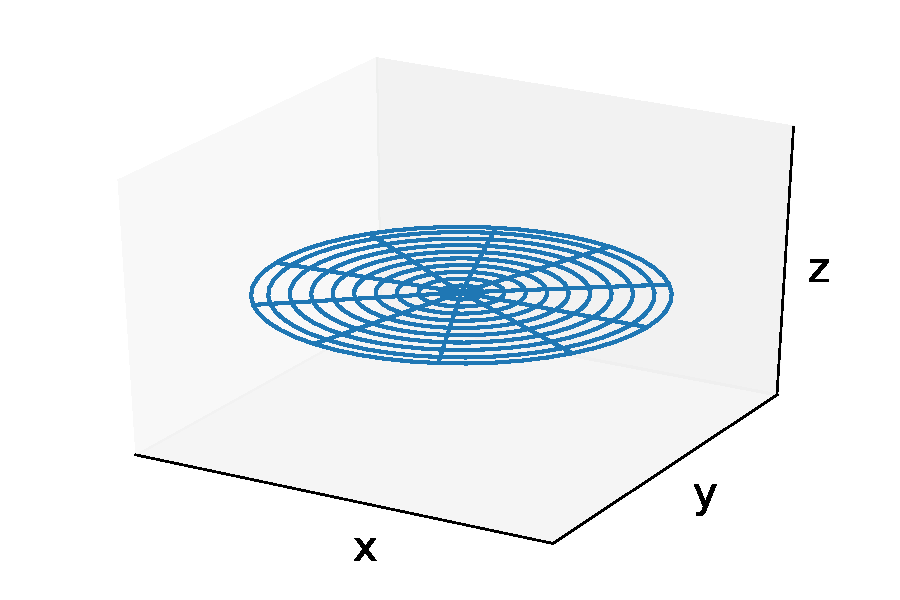
\includegraphics[width=0.8\linewidth]{TCFE_4/membrana.pdf}
\caption{Representação da membrana circular}
\end{figure}

\section*{Equação da Onda Bi-Dimensional}
Aferem-se agora as consequências das suposições físicas na força de tensão presente num pedaço da membrana.
\subsection*{Componente Horizontal}
As componentes horizontais obtém-se através do produto do módulo da força com o coseno do ângulo de inclinação. Para pequenos deslocamentos pode-se aproximar o coseno a 1, pelo que as forças opostas cancelam-se. A componente horizontal da tensão é, portanto, nula.

\subsection*{Componente Vertical}
As componentes verticais da força de tensão para uma pequena secção quadrada da membrana, representada na figura \ref{esquema}, correspondem a:

\vspace{-0.4cm}
\begin{align*}
 -T \Delta y\sin{(\alpha)} & & T \Delta y\sin{(\beta)}
\end{align*}

Usando a aproximação da tangente, uma vez que os ângulos de inclinação são pequenos, a tensão resultante é dada por:
\begin{align*}
 T\Delta y(\sin{(\beta)} - \sin{(\alpha)}) &\approx T\Delta y(\tan(\beta) - \tan(\alpha))\\
                                     &= T\Delta y\bigg( \frac{\partial z(x + \Delta x, y_1)}{\partial x} - \frac{\partial z(x, y_2)}{\partial x}\bigg)
\end{align*}
onde $y_1$, $y_2$ $\in$ ]$y$, $y+ \Delta y$[

\pagebreak

por simetria, para $T\Delta x$ tem-se:

\vspace{-0.4cm}

\begin{align*}
 T\Delta x(\sin(\beta) - \sin(\alpha)) \approx T\Delta x\bigg( \frac{\partial z(x_1, y + \Delta y)}{\partial x} - \frac{\partial z(x_2, y)}{\partial x}\bigg)
\end{align*}
onde $x_1$, $x_2$ $\in$ ]$x$, $x+ \Delta x$[ \par

Da 2ª lei de Newton e uma vez que os deslocamentos são transversais, vem:

\begin{align*}
    \rho \Delta A \frac{\partial^2{z}}{\partial{t^2}} = \rho \Delta x \Delta y \frac{\partial^2{z}}{\partial{t^2}} &= T\Delta x\bigg( \frac{\partial z(x_1, y + \Delta y)}{\partial x} - \frac{\partial z(x_2, y)}{\partial x}\bigg) \\
     &+ T\Delta y\bigg( \frac{\partial z(x + \Delta x, y_1)}{\partial x} - \frac{\partial z(x, y_2)}{\partial x}\bigg)
\end{align*}

No limite $\Delta x \longrightarrow 0$ e $\Delta y\longrightarrow 0$, resulta a equação de onda a 2 dimensões:

\begin{equation}
    \frac{\partial^2{z}}{\partial{t^2}} = c^2 \nabla^2z \hspace{0.5 cm}  \mbox{onde $c = \frac{T}{\rho}$.}
    \label{func_onda}
\end{equation}
Devido à simetria circular do problema é preferível trabalhar em coordenadas polares. Desta forma o laplaciano é dado por:
\begin{equation*}
    \nabla^2z=\frac{\partial^2{z}}{\partial{r^2}} +\frac{1}{r}\frac{\partial{z}}{\partial{r}} + \frac{1}{r^2}\frac{\partial^2{z}}{\partial{\theta^2}} 
\end{equation*}

\vspace{-0.55cm}

\begin{figure}[ht]
\centering
\captionsetup{justification=centering}
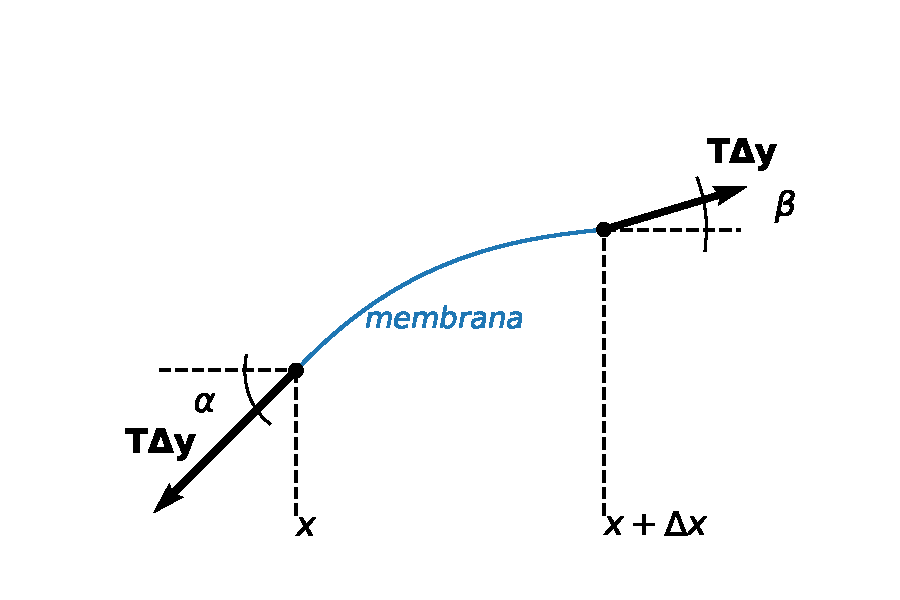
\includegraphics[width=0.8\linewidth]{TCFE_4/horizontal.pdf}
\caption{secção de membrana no plano $xz$}
\label{esquema}
\end{figure}

\section*{Caso Geral}
Pelo método da separação de variáveis, tem-se:
\begin{equation}
    z(r,\theta,t) = R(r)\cdot \Theta(\theta)\cdot T(t)
    \label{geral}
\end{equation}
Substituindo em \ref{func_onda} resulta:

\begin{equation*}
    \begin{cases} \frac{T''(t)}{c^2T(t)} = -\lambda^2 \\
    \\
    \frac{R''(r)}{R(r)} + \frac{R'(r)}{rR(r)} + \frac{\Theta''(\theta}{r^2\Theta(\theta)} = -\lambda^2 \end{cases}
\end{equation*}
Pelo que a solução de $T(t)$ é dada por uma combinação linear de senos e cossenos:

\begin{equation*}
    T(t) = A\cos(c\lambda t) + B\sin(c\lambda t)
\end{equation*}
 multiplicando por $r^2$ e separando as variáveis da equação dependente de $\theta$ e $r$, obtem-se:
 
 \begin{equation*}
    \begin{cases} \lambda^2r^2 + \frac{r^2R''(r)}{R(r)} + \frac{rR'(r)}{R(r)}= L \\
    \\
    -\frac{\Theta''(\theta)}{\Theta(\theta)} = L\end{cases}
\end{equation*}

Desta forma, a solução de $\Theta(\theta)$ é dada por:

\begin{equation*}
    \Theta(\theta) = C\cos(m\theta) + D\sin(m\theta) \hspace{0.5 cm}  \mbox{L = $m^2$ e $m$ = 0, 1, ...}
\end{equation*}

A solução de $R(r)$ é uma combinação linear das funções de Bessel $J_m$ e $Y_m$, assumindo a forma:

\begin{equation*}
    R(r) = J_m(\lambda_{mn}r) \hspace{0.5 cm}  \mbox{m = 0, 1, ... e n = 1, 2, ...}
\end{equation*}
onde $\lambda_{mn}$ = $\alpha_{mn}/a$, sendo que $a_{mn}$ corresponde a raiz $n$ positiva da função $J_m$.\par
Substituindo as soluções de $R(r)$, $\Theta(\theta)$ e $T(t)$ na equação \ref{geral}, obtem-se a solução geral do problema.
 
 \section*{Simulação Computacional}
 A simulação dos modos normais da pele do bongo de Feynmann foi implementada em \textit{Python}, tendo sido utilizado o ambiente \textit{Jupyter Notebook}, que permite uma execução do código rápida.
\par Utilizaram-se as bibliotecas de cálculo: \textit{numpy} e \textit{scipy}, sendo que a última contém já definidas as funções de Bessel e as suas raizes. A parte gráfica baseou-se na biblioteca \textit{matplotlib}, nomeadamente a extensão que permite a visualização tri-dimensional, que foi utilizada para simular superfície da membrana. Foi também traçado um corte horizontal da membrana, na base da mesma.

Utilizaram-se os seguintes valores arbitrários na solução geral:
\begin{center}
$A = 0s$, $B = 1s$, $C = 1$ e $D = 0$.\\
$a = 1m$, $c = 0.75 ms^{-1}$ e $t = 0s$.
\end{center}
Encontram-se à direita uma representação dos primeiros modos normais obtidos na simulação da membrana, correspondendo da esquerda para a direita a:

\begin{align*}
    z_{mn} = &\{ (0, 1), (0, 2), (0, 3)\\
             &   \hspace{0.2cm} (1, 1), (1, 2), (1, 3)\\
             &   \hspace{0.2cm} (2, 1), (2, 2), (2, 3)\}
\end{align*}

\section*{Discussão dos Resultados}

O corte horizontal facilita a visualização das componentes radiais e angulares de cada modo de vibração, sendo possível observar as simetrias de $\theta$ e $r$.\par
Para $n$, observam-se $n$ 'fatias' da membrana, formando angulos de $\frac{2\pi}{n}$, quando $n>0$.
Para $m$, observam-se $m$ circunferências contidas dentro da circunferência de raio $a$.
\par 

%------------------------------------------------Adds this section to the table of contents

%----------------------------------------------------------------------------------------
%	REFERENCE LIST
%----------------------------------------------------------------------------------------


\begin{thebibliography}{9}
\bibitem{}
\label{batuque}
\url{https://www.youtube.com/watch?v=HKTSaezB4p8}
\bibitem{guia} 
\url{https://en.wikipedia.org/wiki/Vibrations\_of\_a\_circular\_membrane}
\bibitem{}
\url{https://en.wikipedia.org/wiki/Bessel_function}
\bibitem{} 
\url{http://zeta.math.utsa.edu/~gokhman/courses/mat3623/Membrane.pdf}
\bibitem{}
\url{https://matplotlib.org/3.2.2/contents.html}
\bibitem{}
\url{https://numpy.org/doc/}
\bibitem{}
\url{https://docs.scipy.org/doc/}

\end{thebibliography}

\vspace{-5cm}
\begin{figure}[]

\begin{minipage}{.5\linewidth}
\centering
\subfloat{\label{main:a}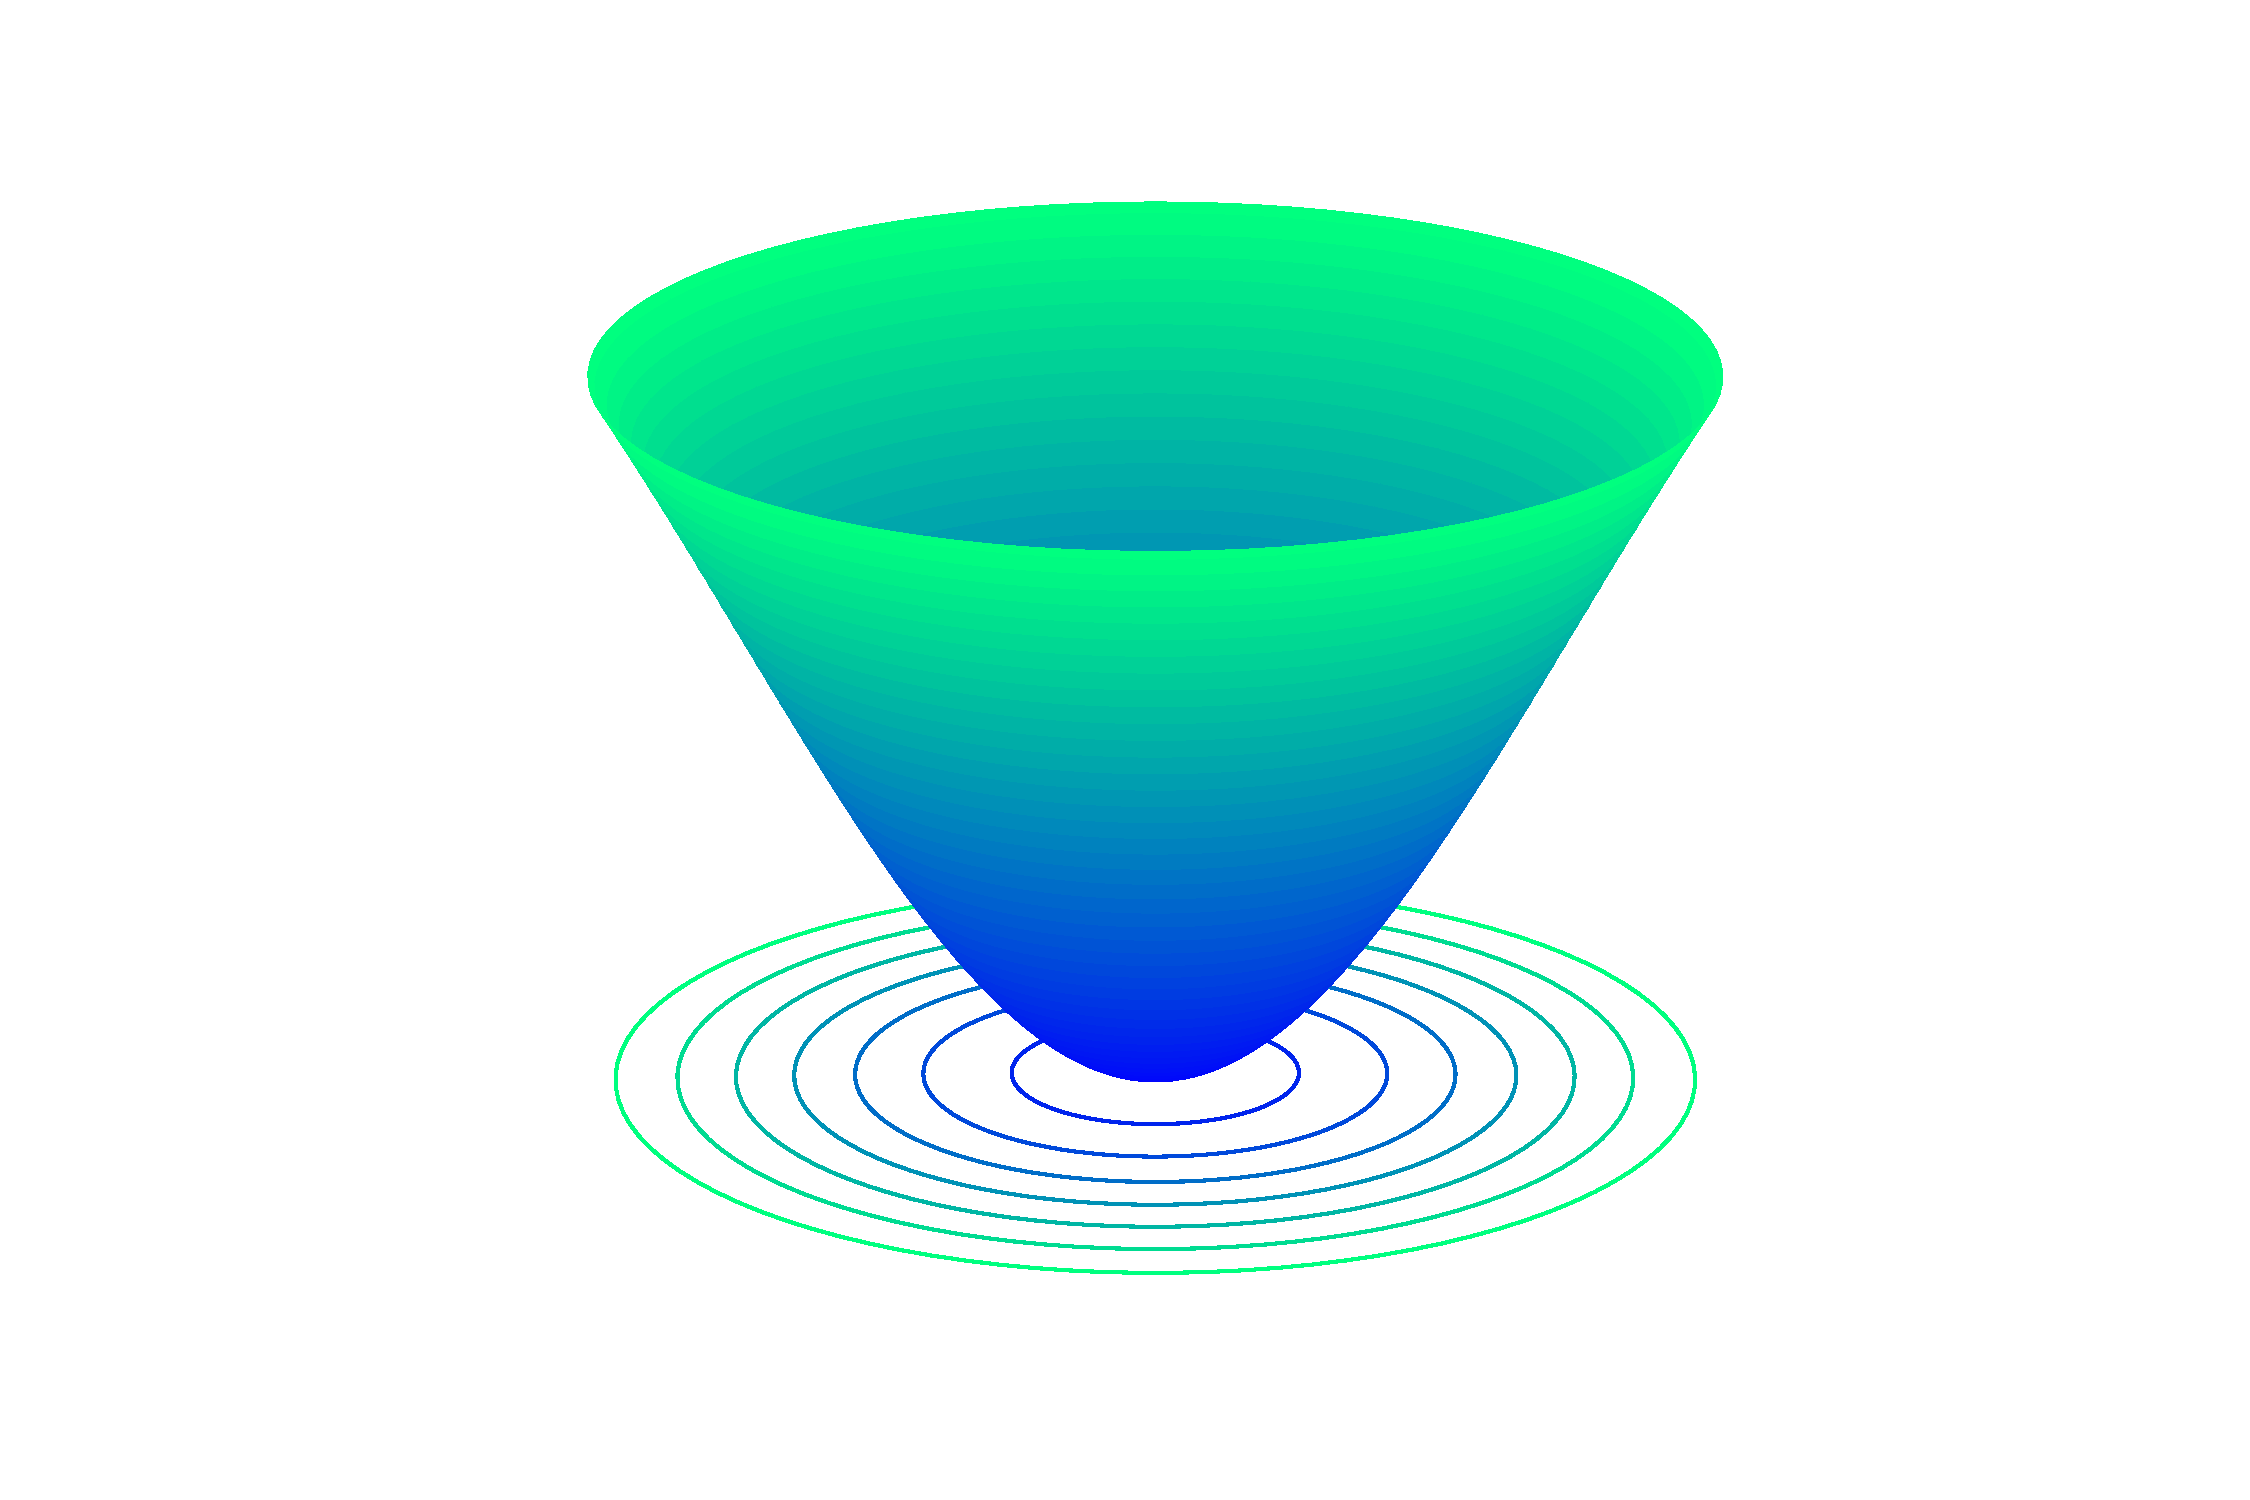
\includegraphics[scale=.16]{TCFE_4/modo_0.pdf}}
\end{minipage}%
\begin{minipage}{.5\linewidth}
\centering
\subfloat{\label{main:b}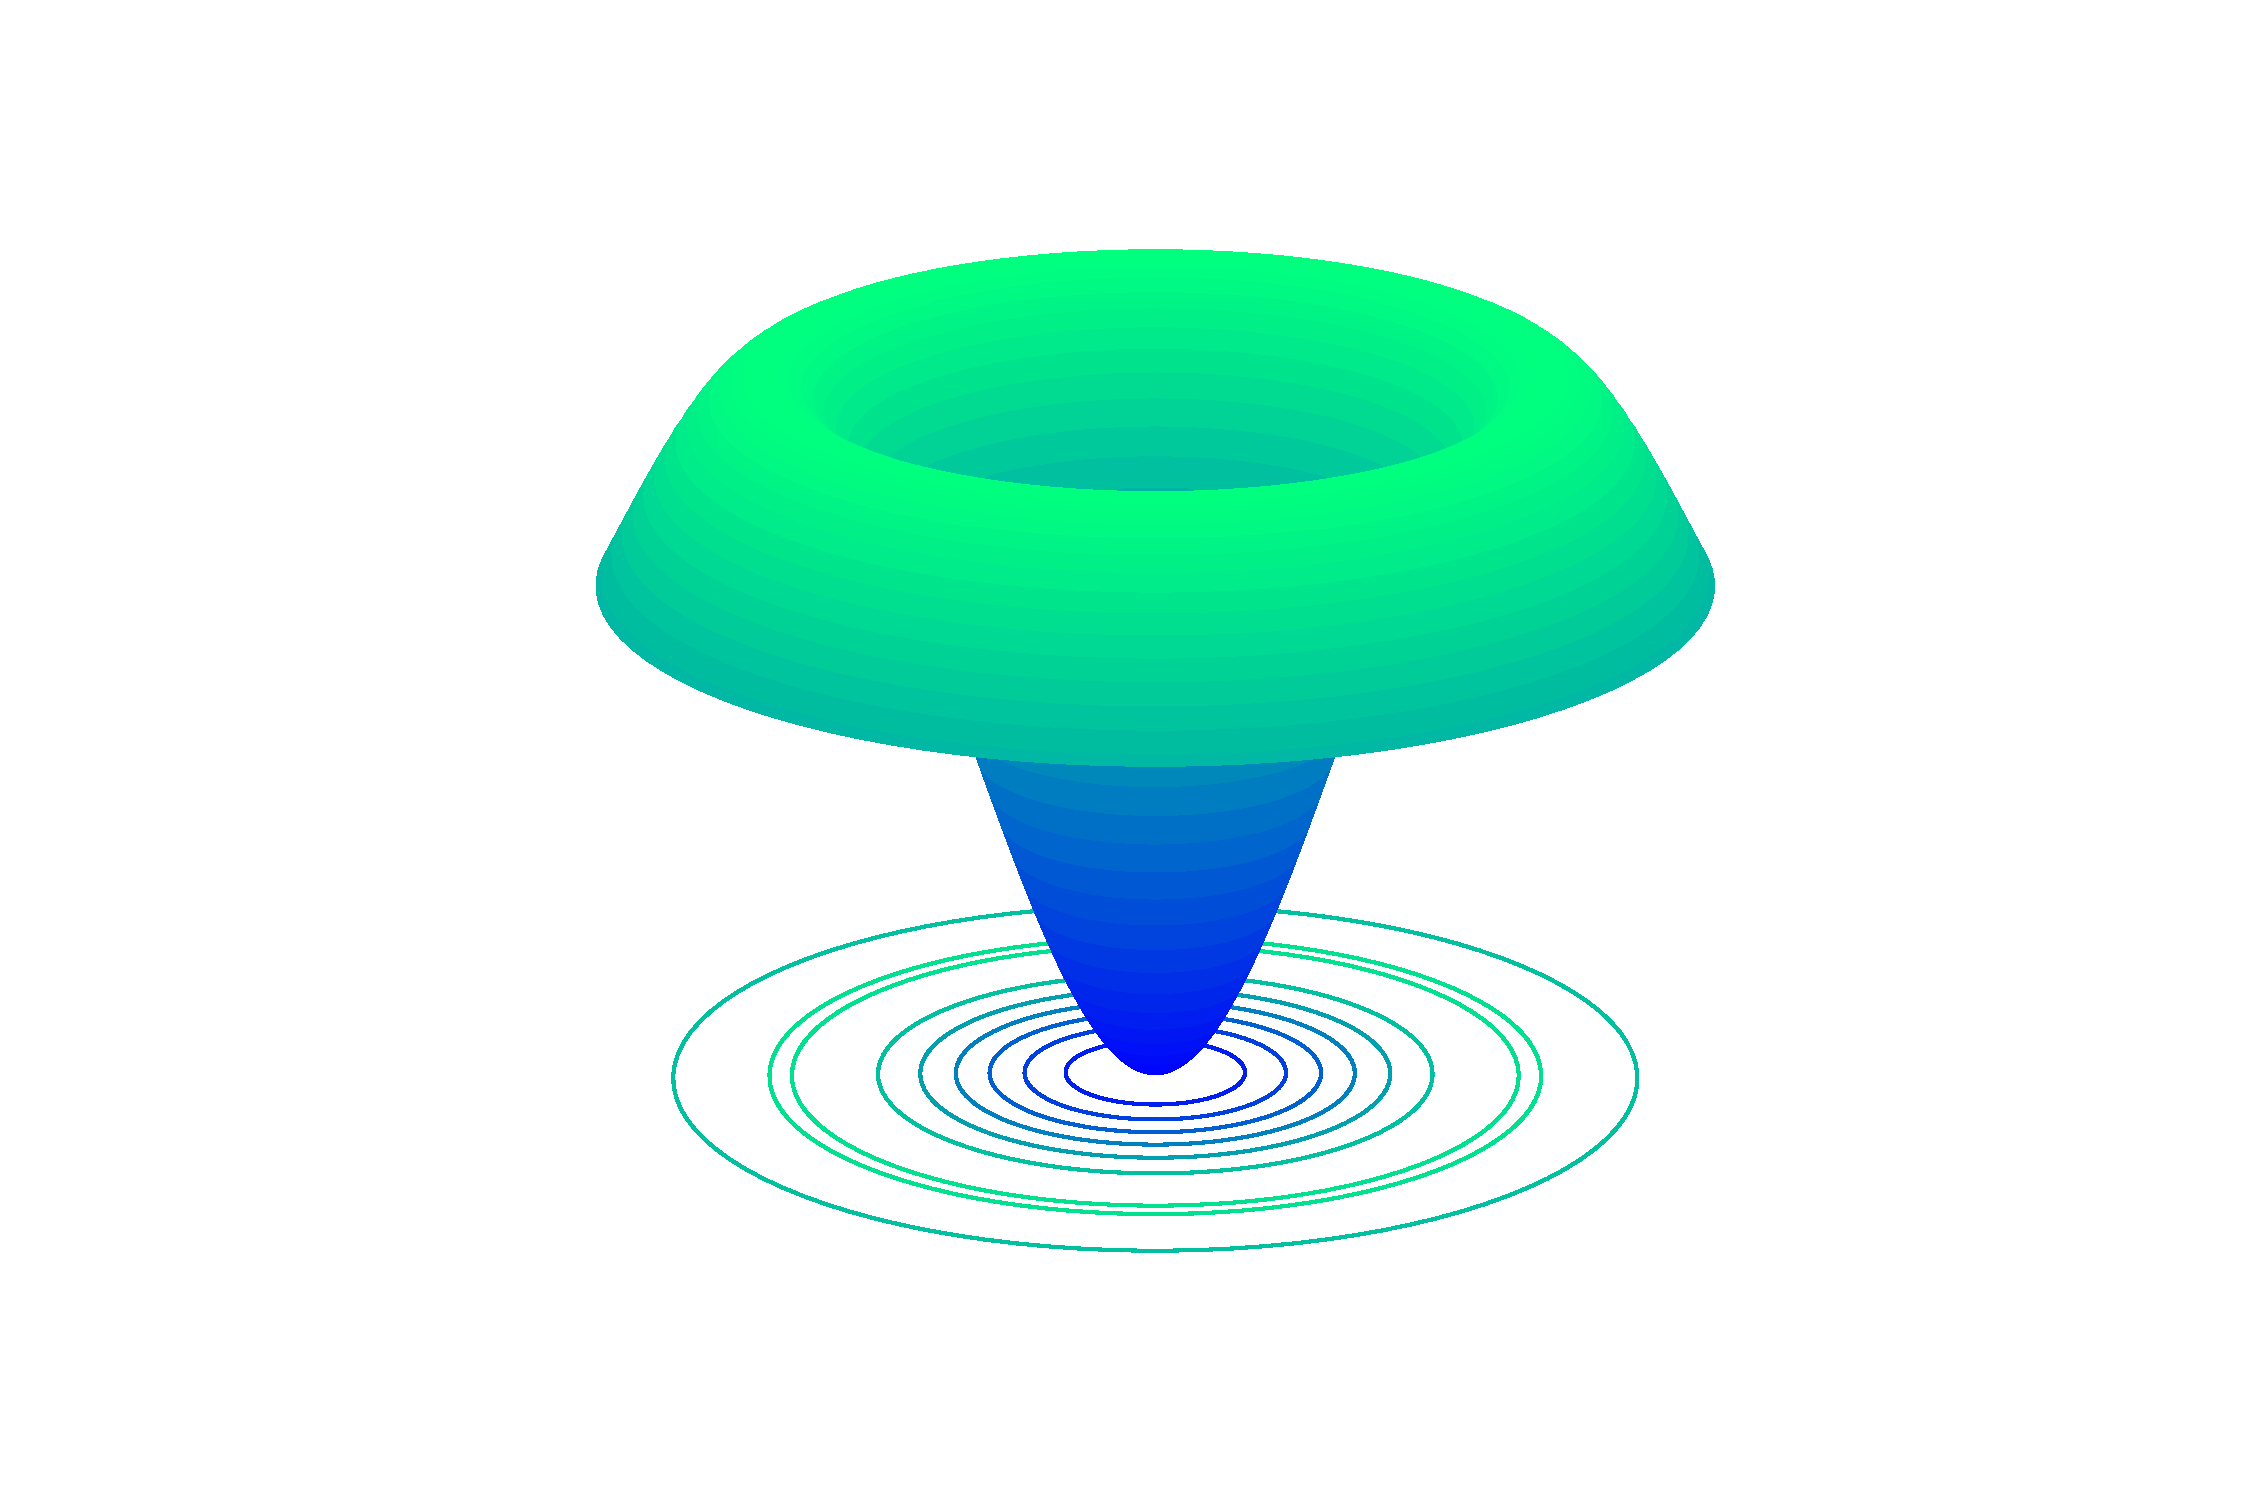
\includegraphics[scale=.16]{TCFE_4/modo_1.pdf}}
\end{minipage}\par\medskip
\centering
\subfloat{\label{main:c}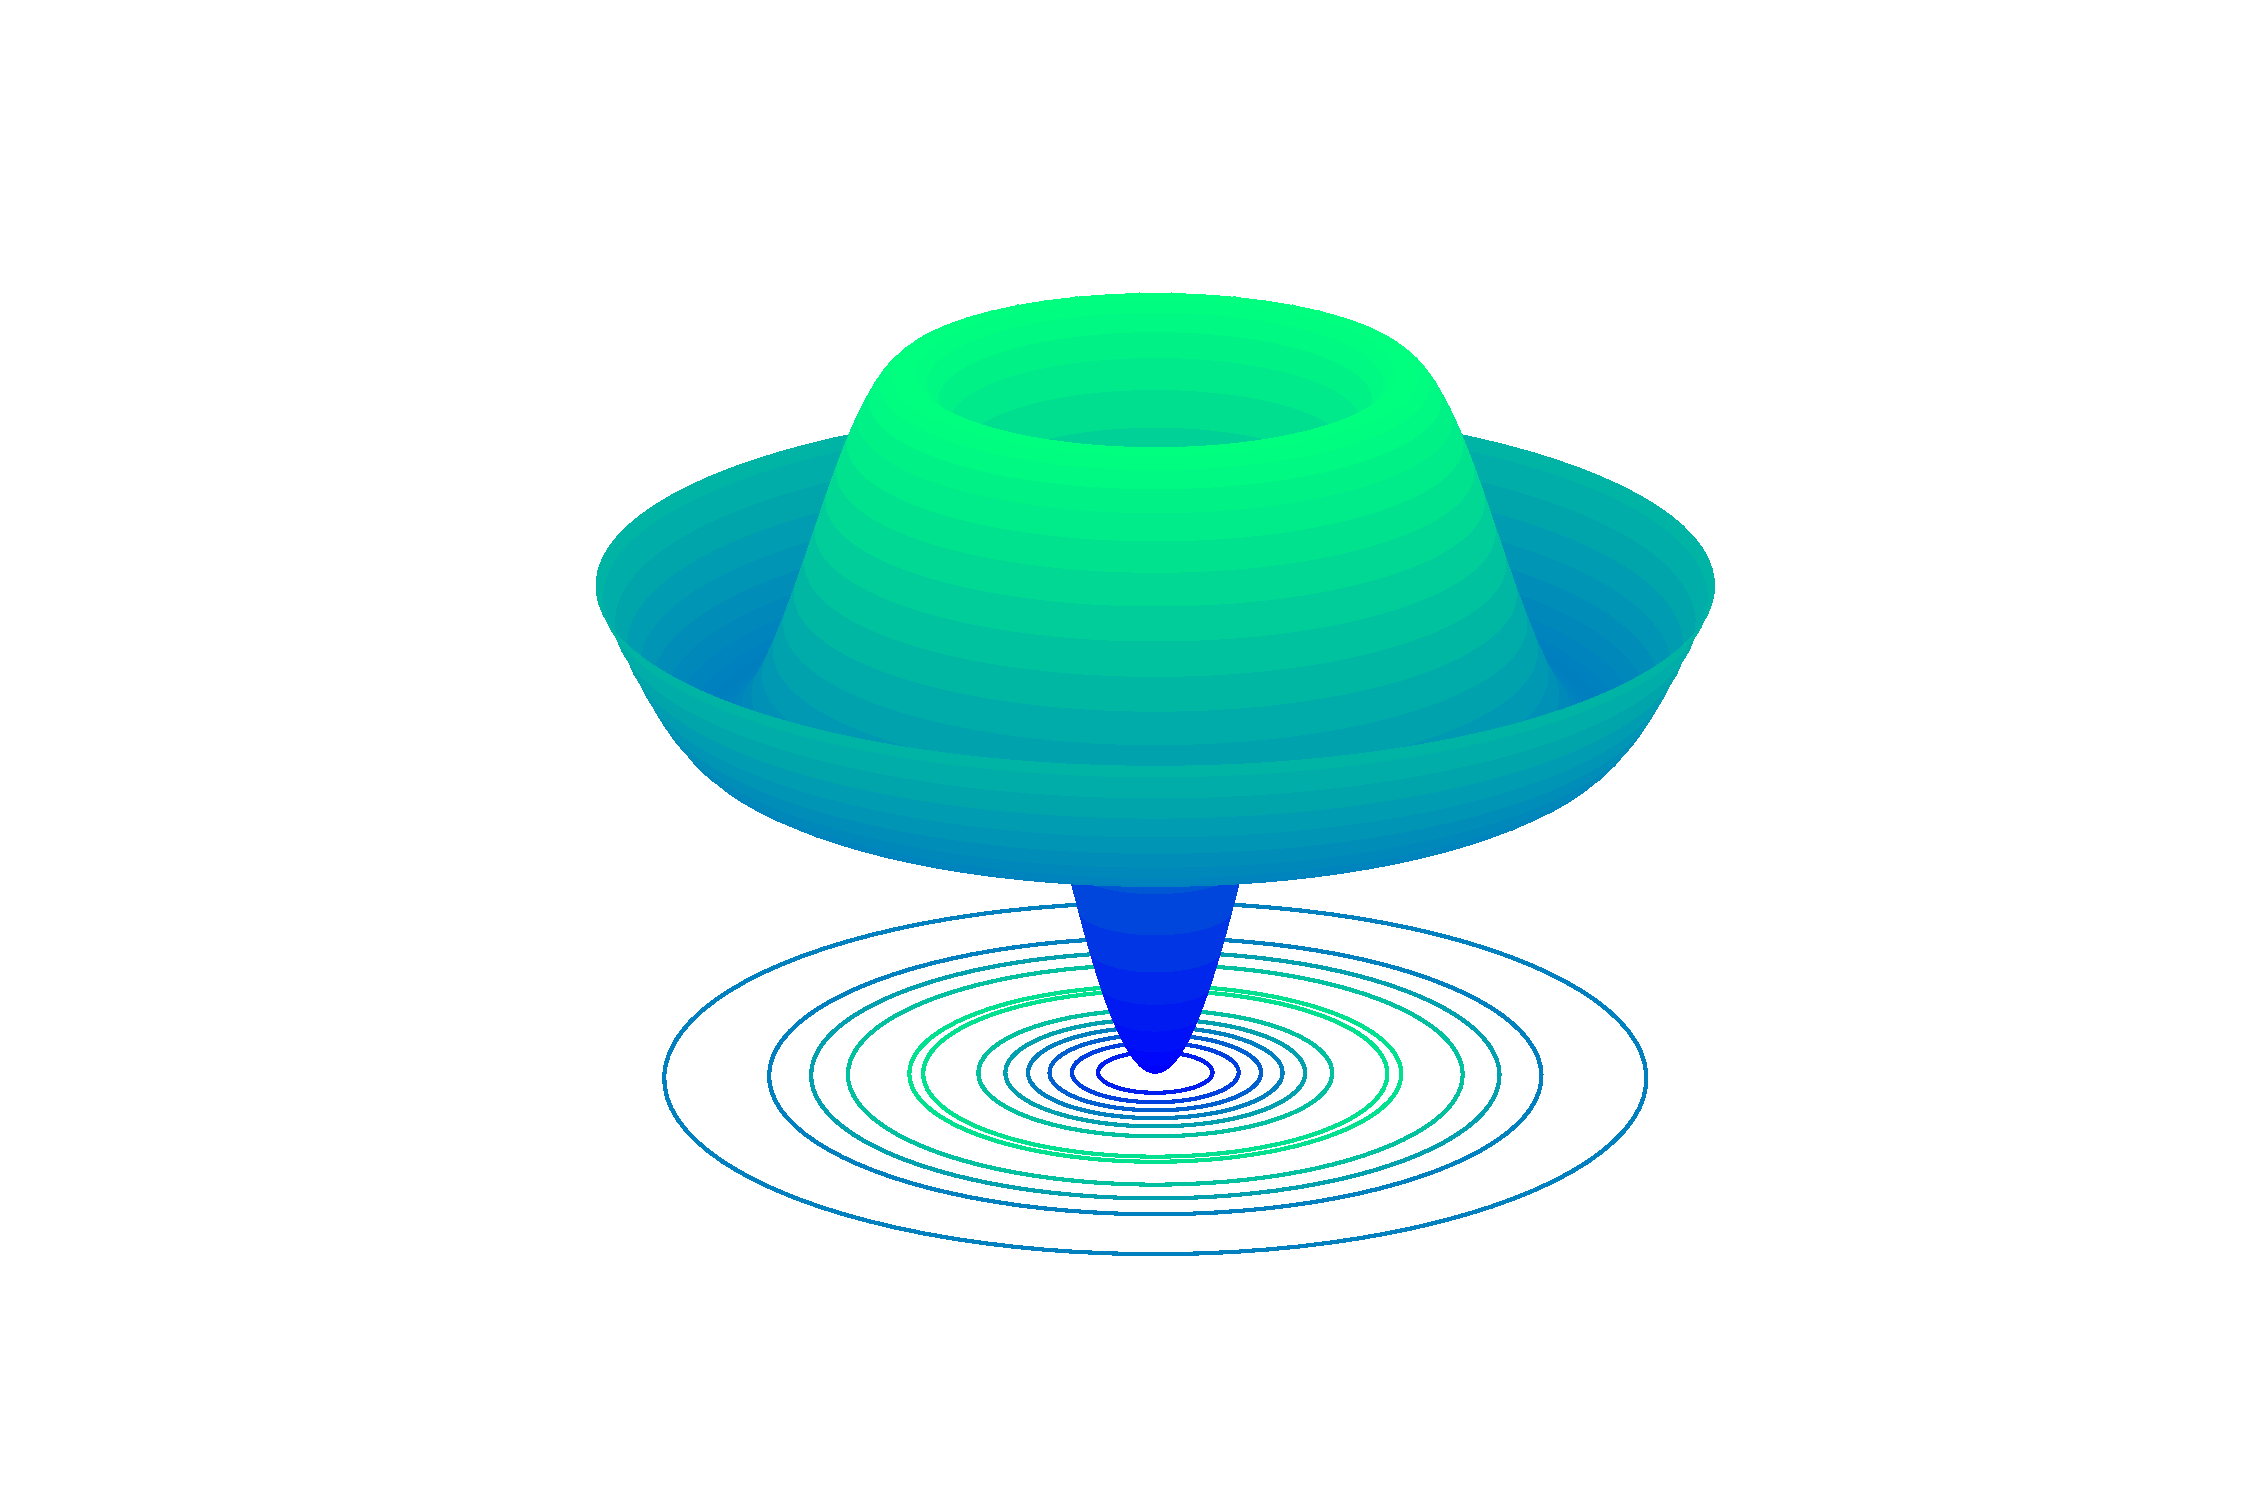
\includegraphics[scale=.16]{TCFE_4/modo_2.pdf}}
\begin{minipage}{.5\linewidth}
\centering
\subfloat{\label{main:a}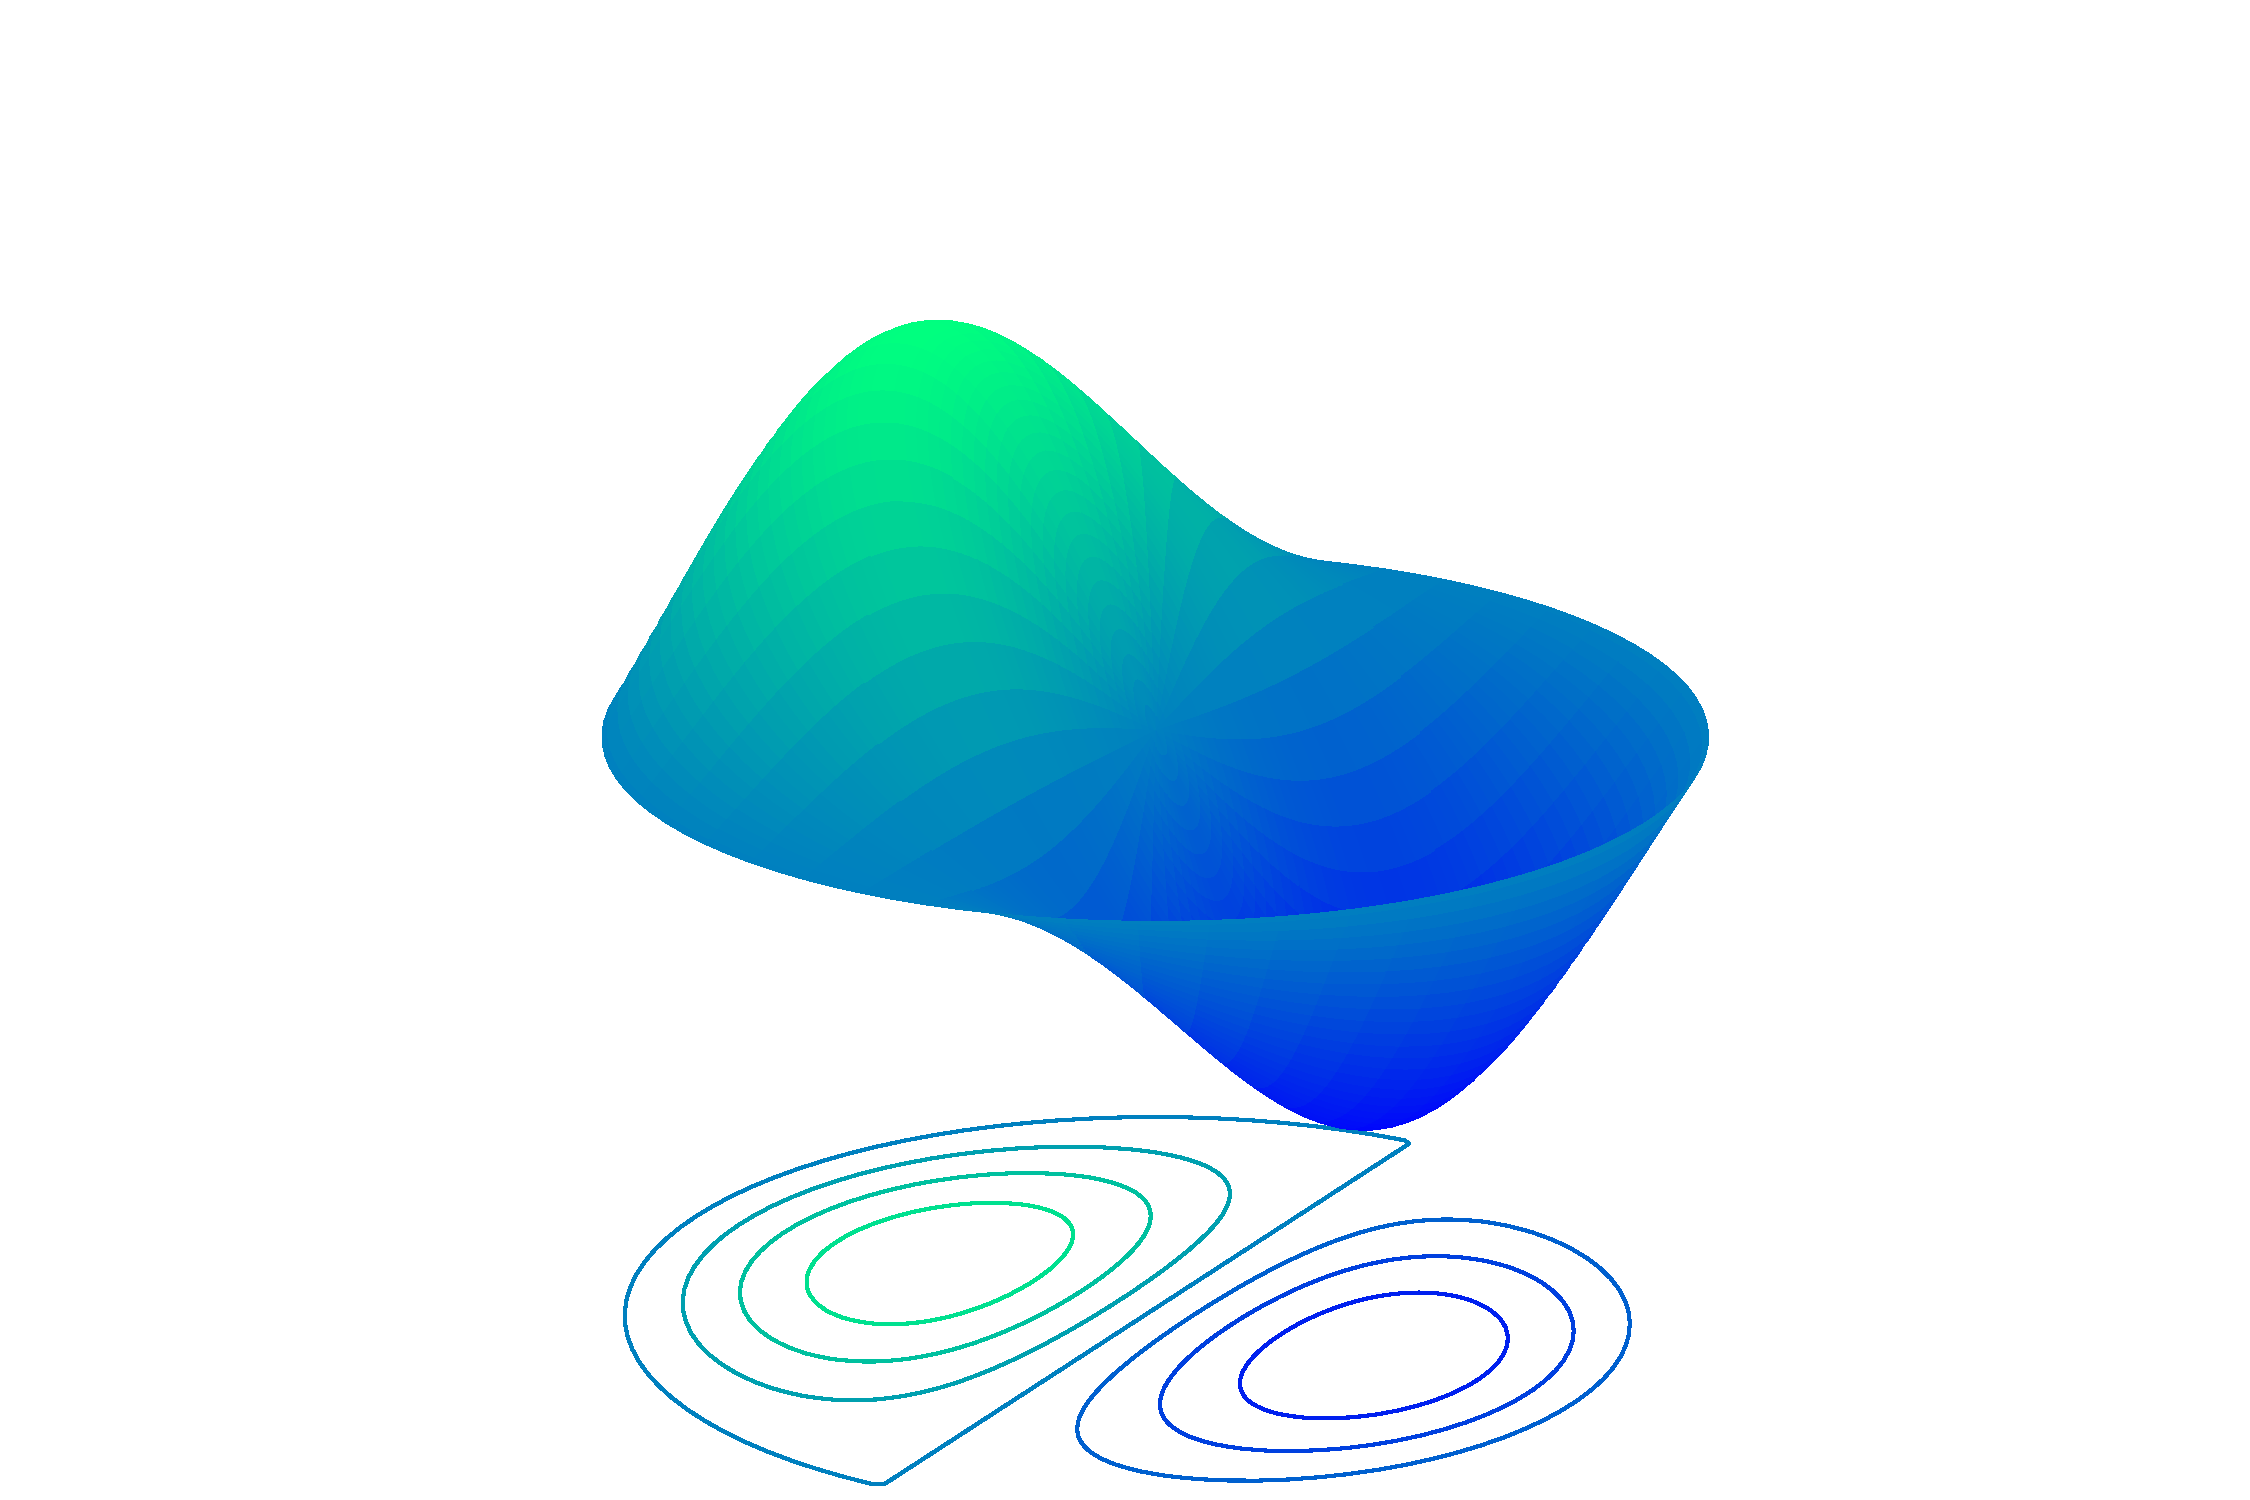
\includegraphics[scale=.16]{TCFE_4/modo_3.pdf}}
\end{minipage}%
\begin{minipage}{.5\linewidth}
\centering
\subfloat{\label{main:b}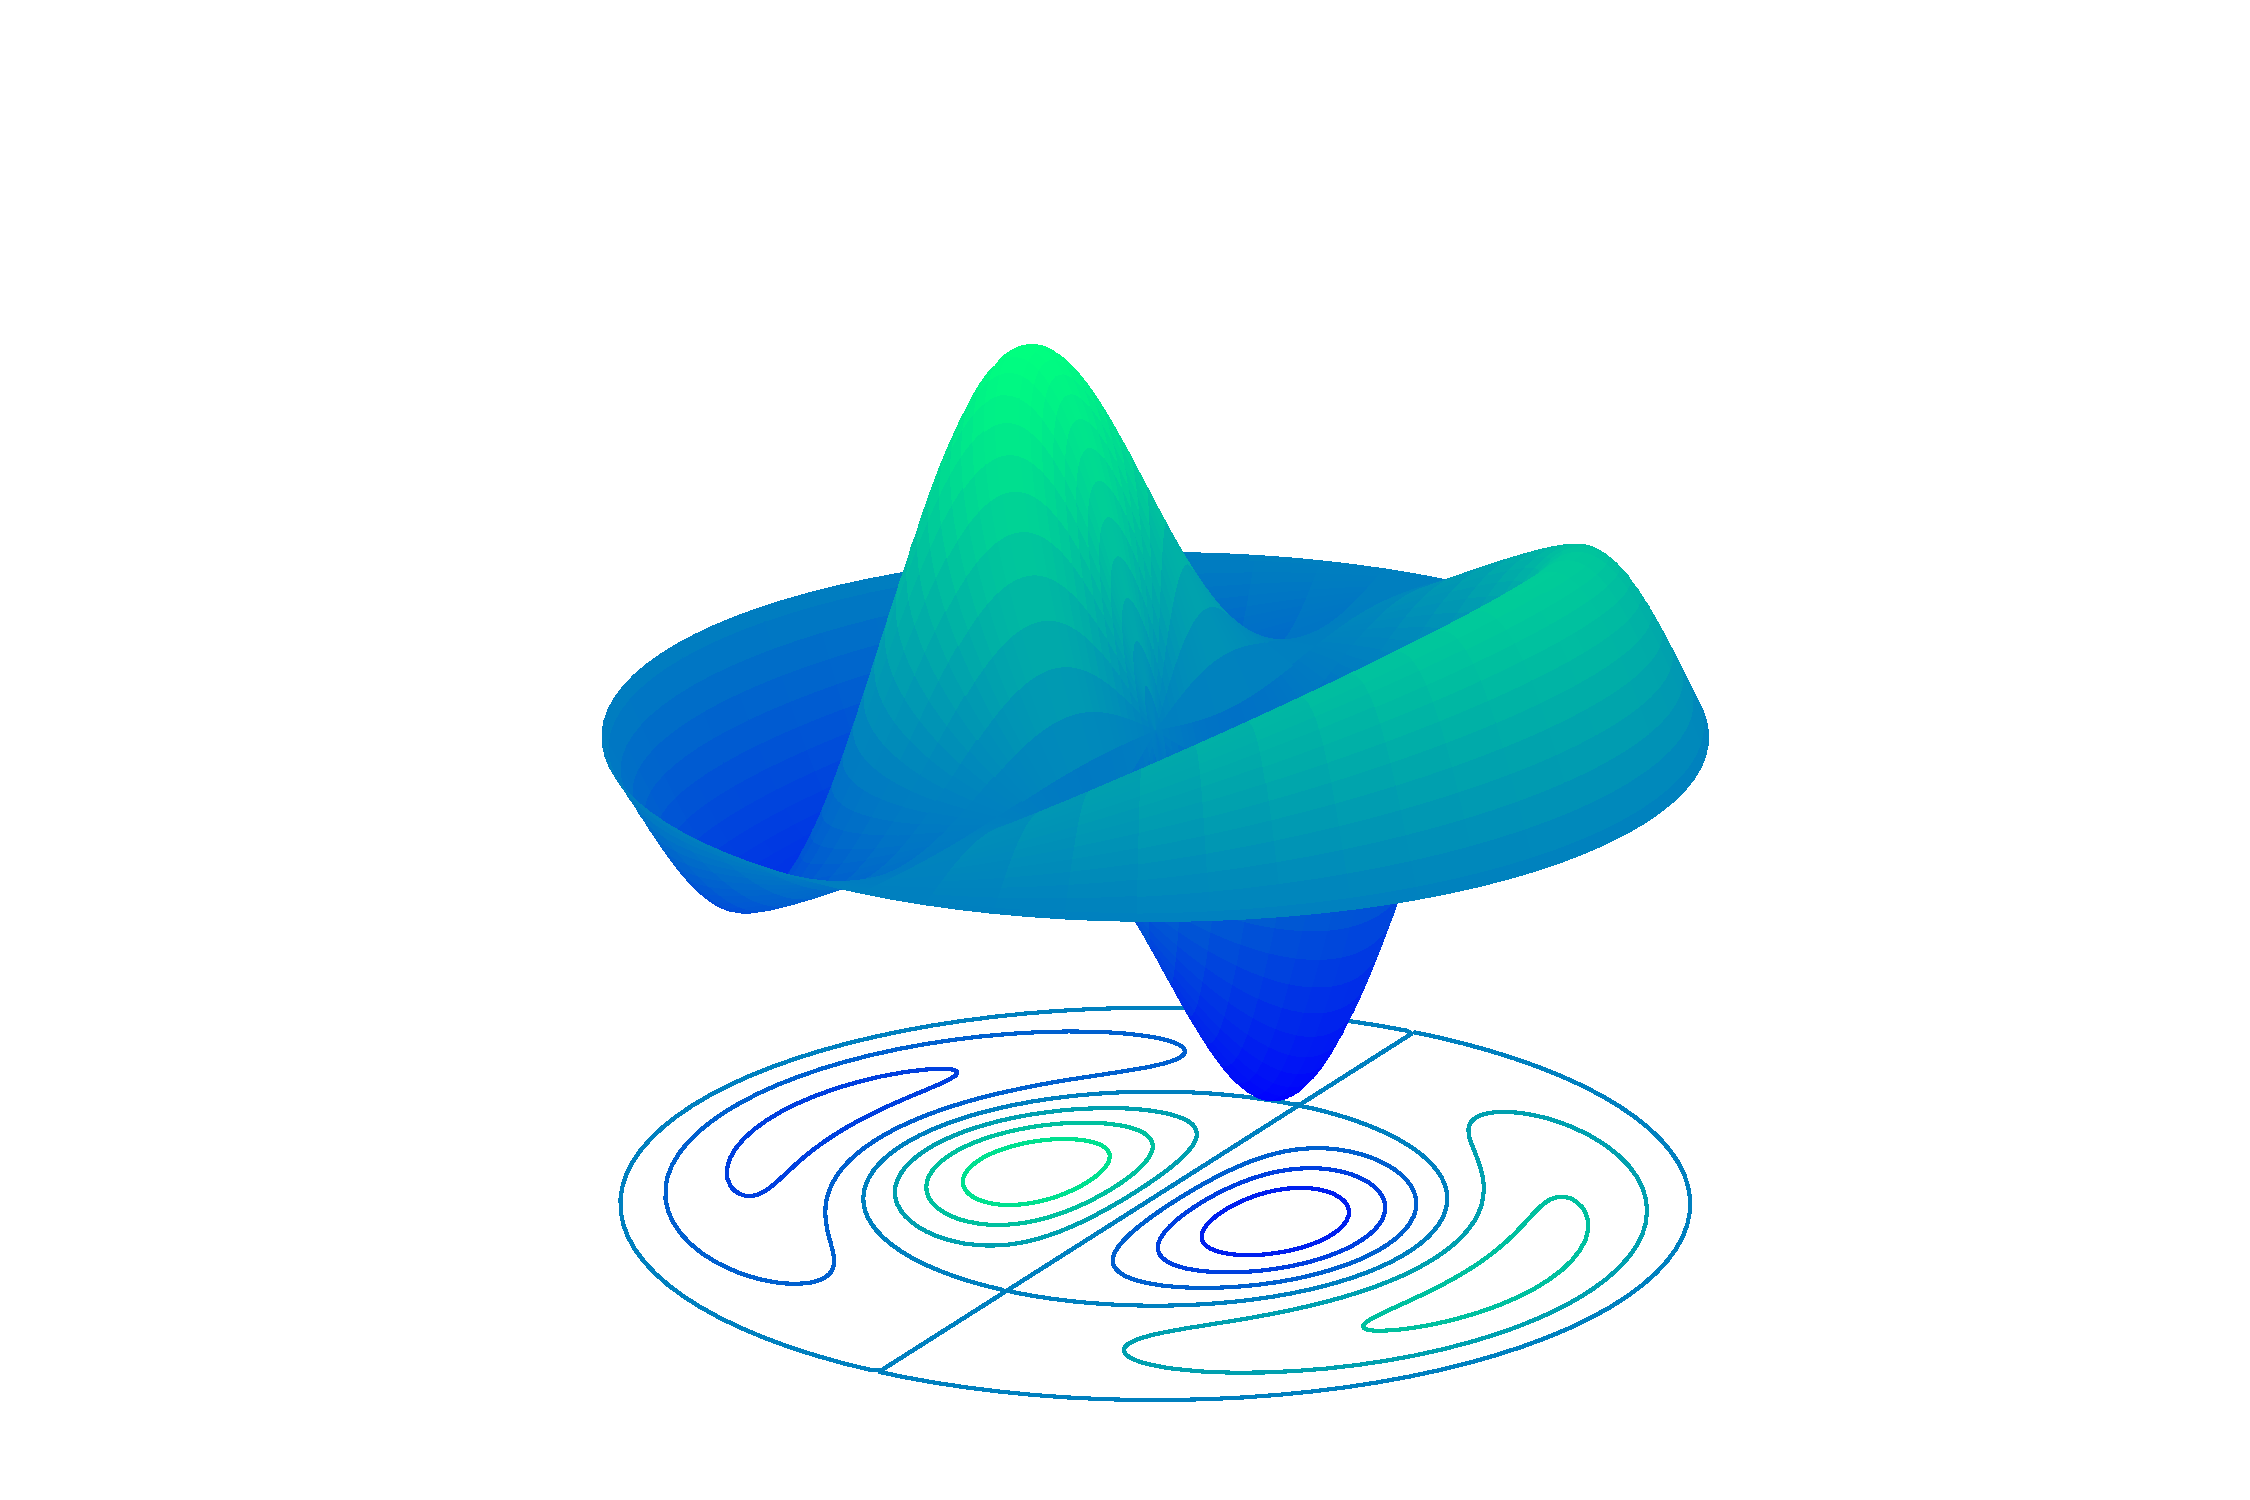
\includegraphics[scale=.16]{TCFE_4/modo_4.pdf}}
\end{minipage}\par\medskip
\centering
\subfloat{\label{main:c}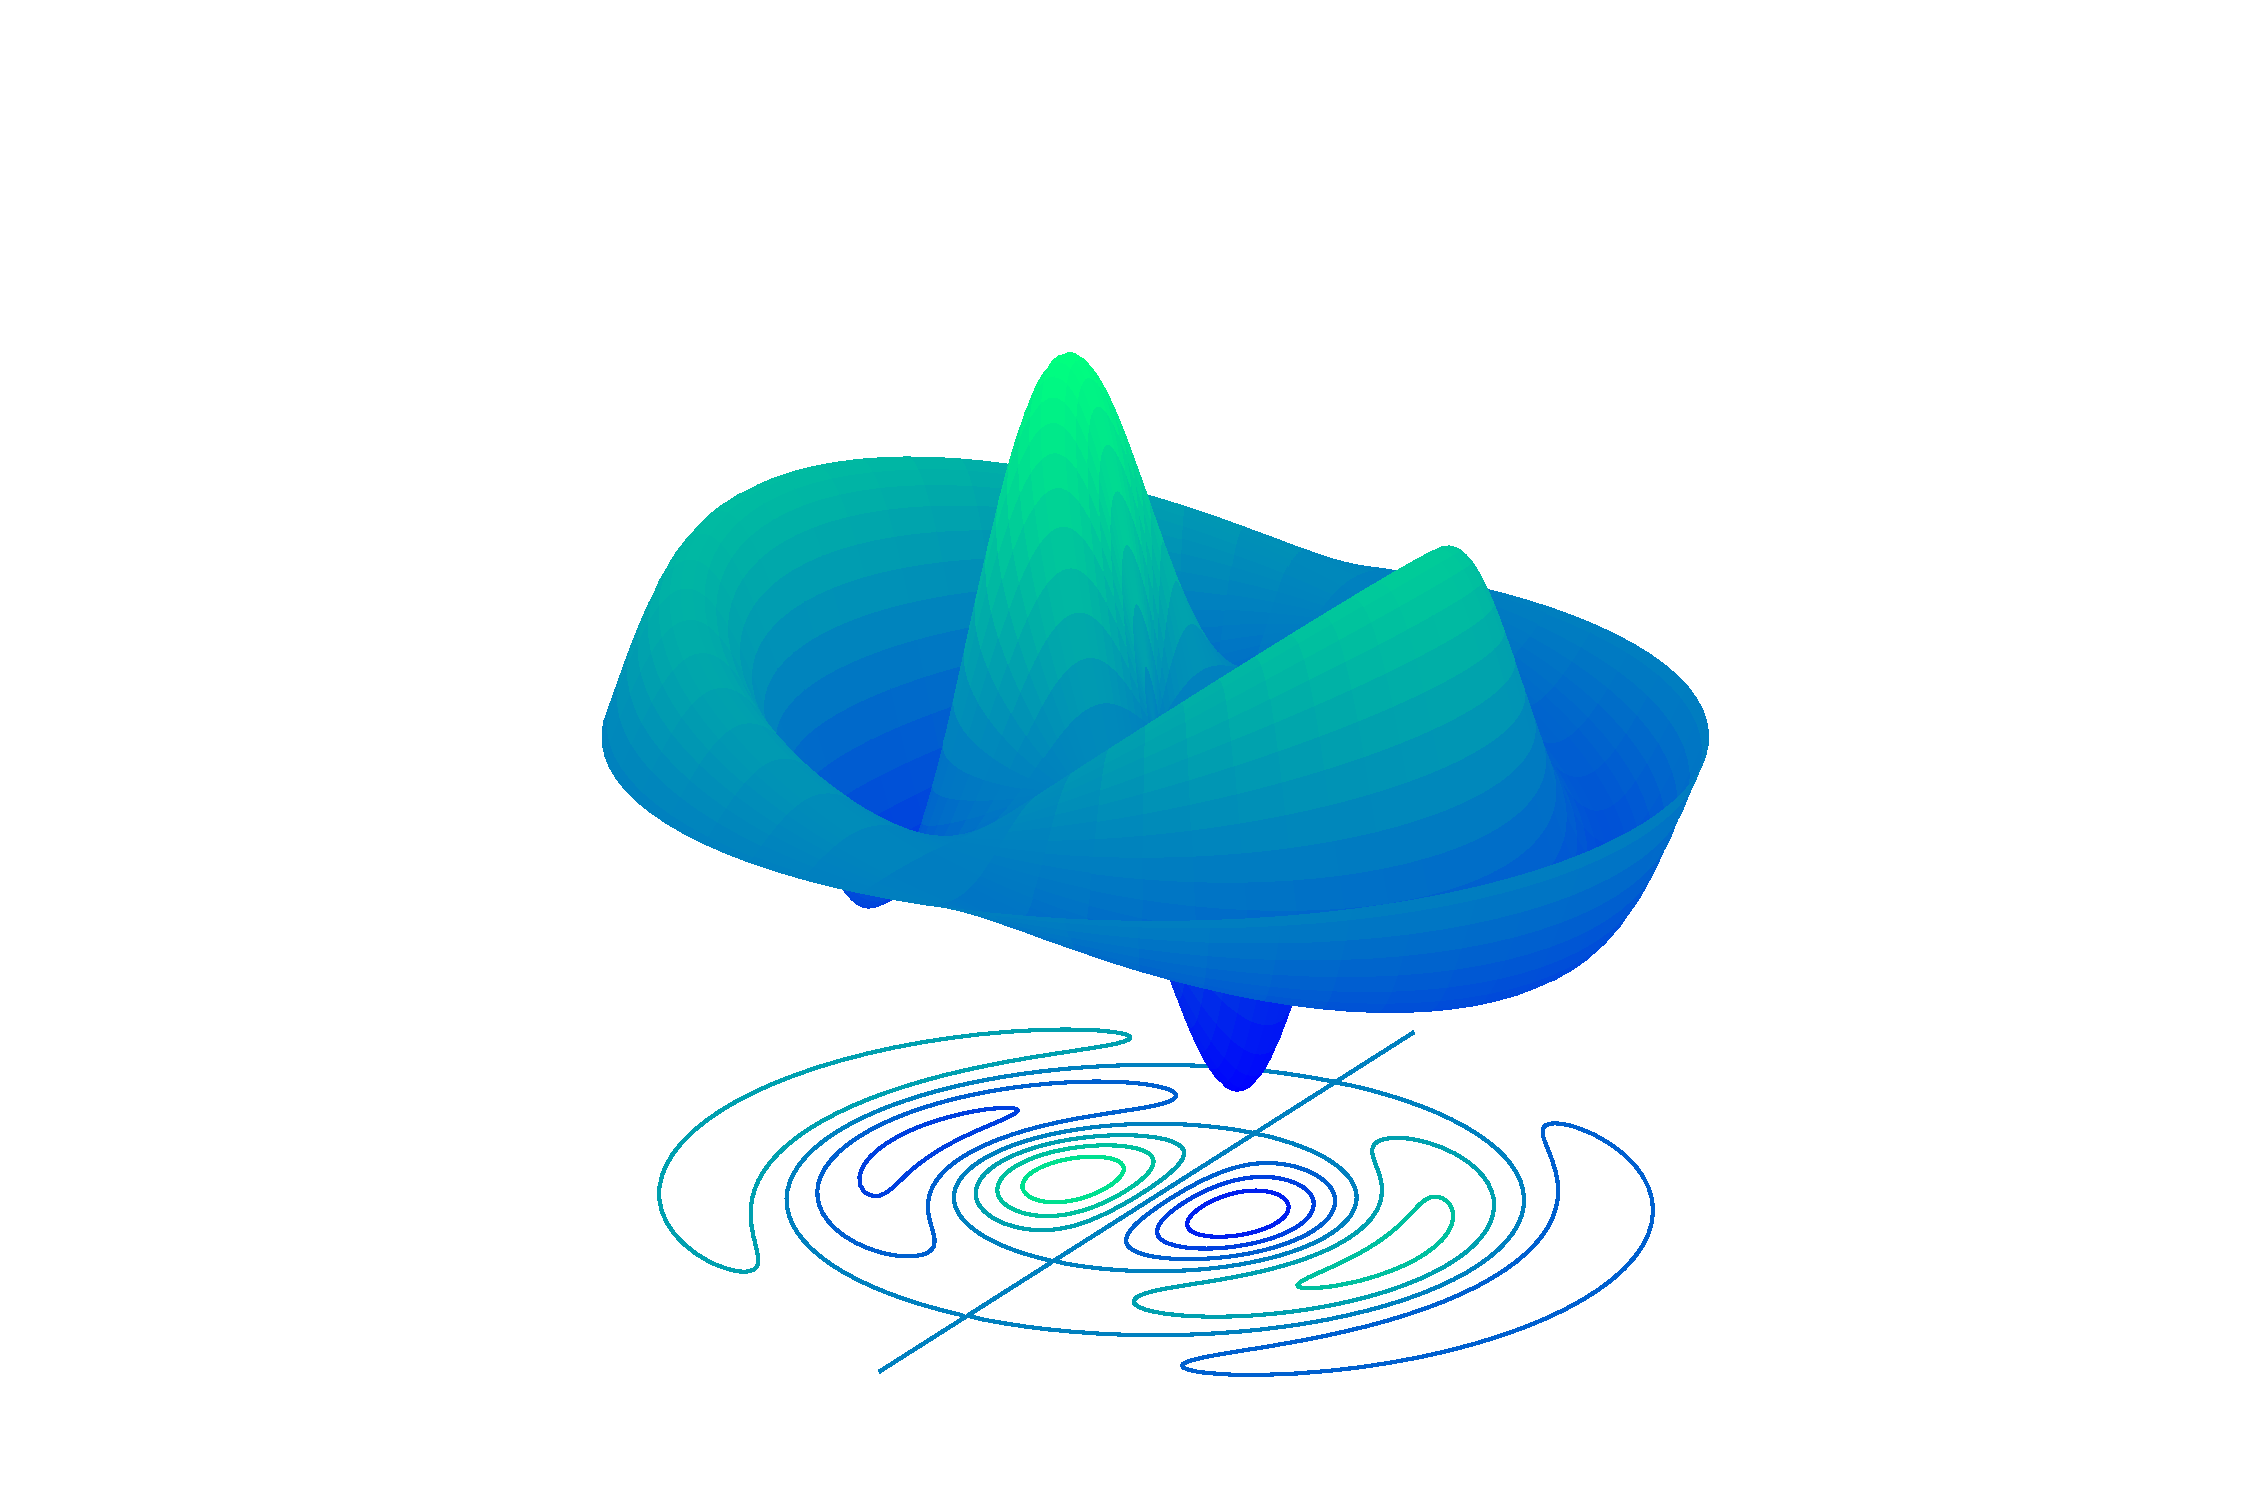
\includegraphics[scale=.16]{TCFE_4/modo_5.pdf}}
\begin{minipage}{.5\linewidth}
\centering
\subfloat{\label{main:a}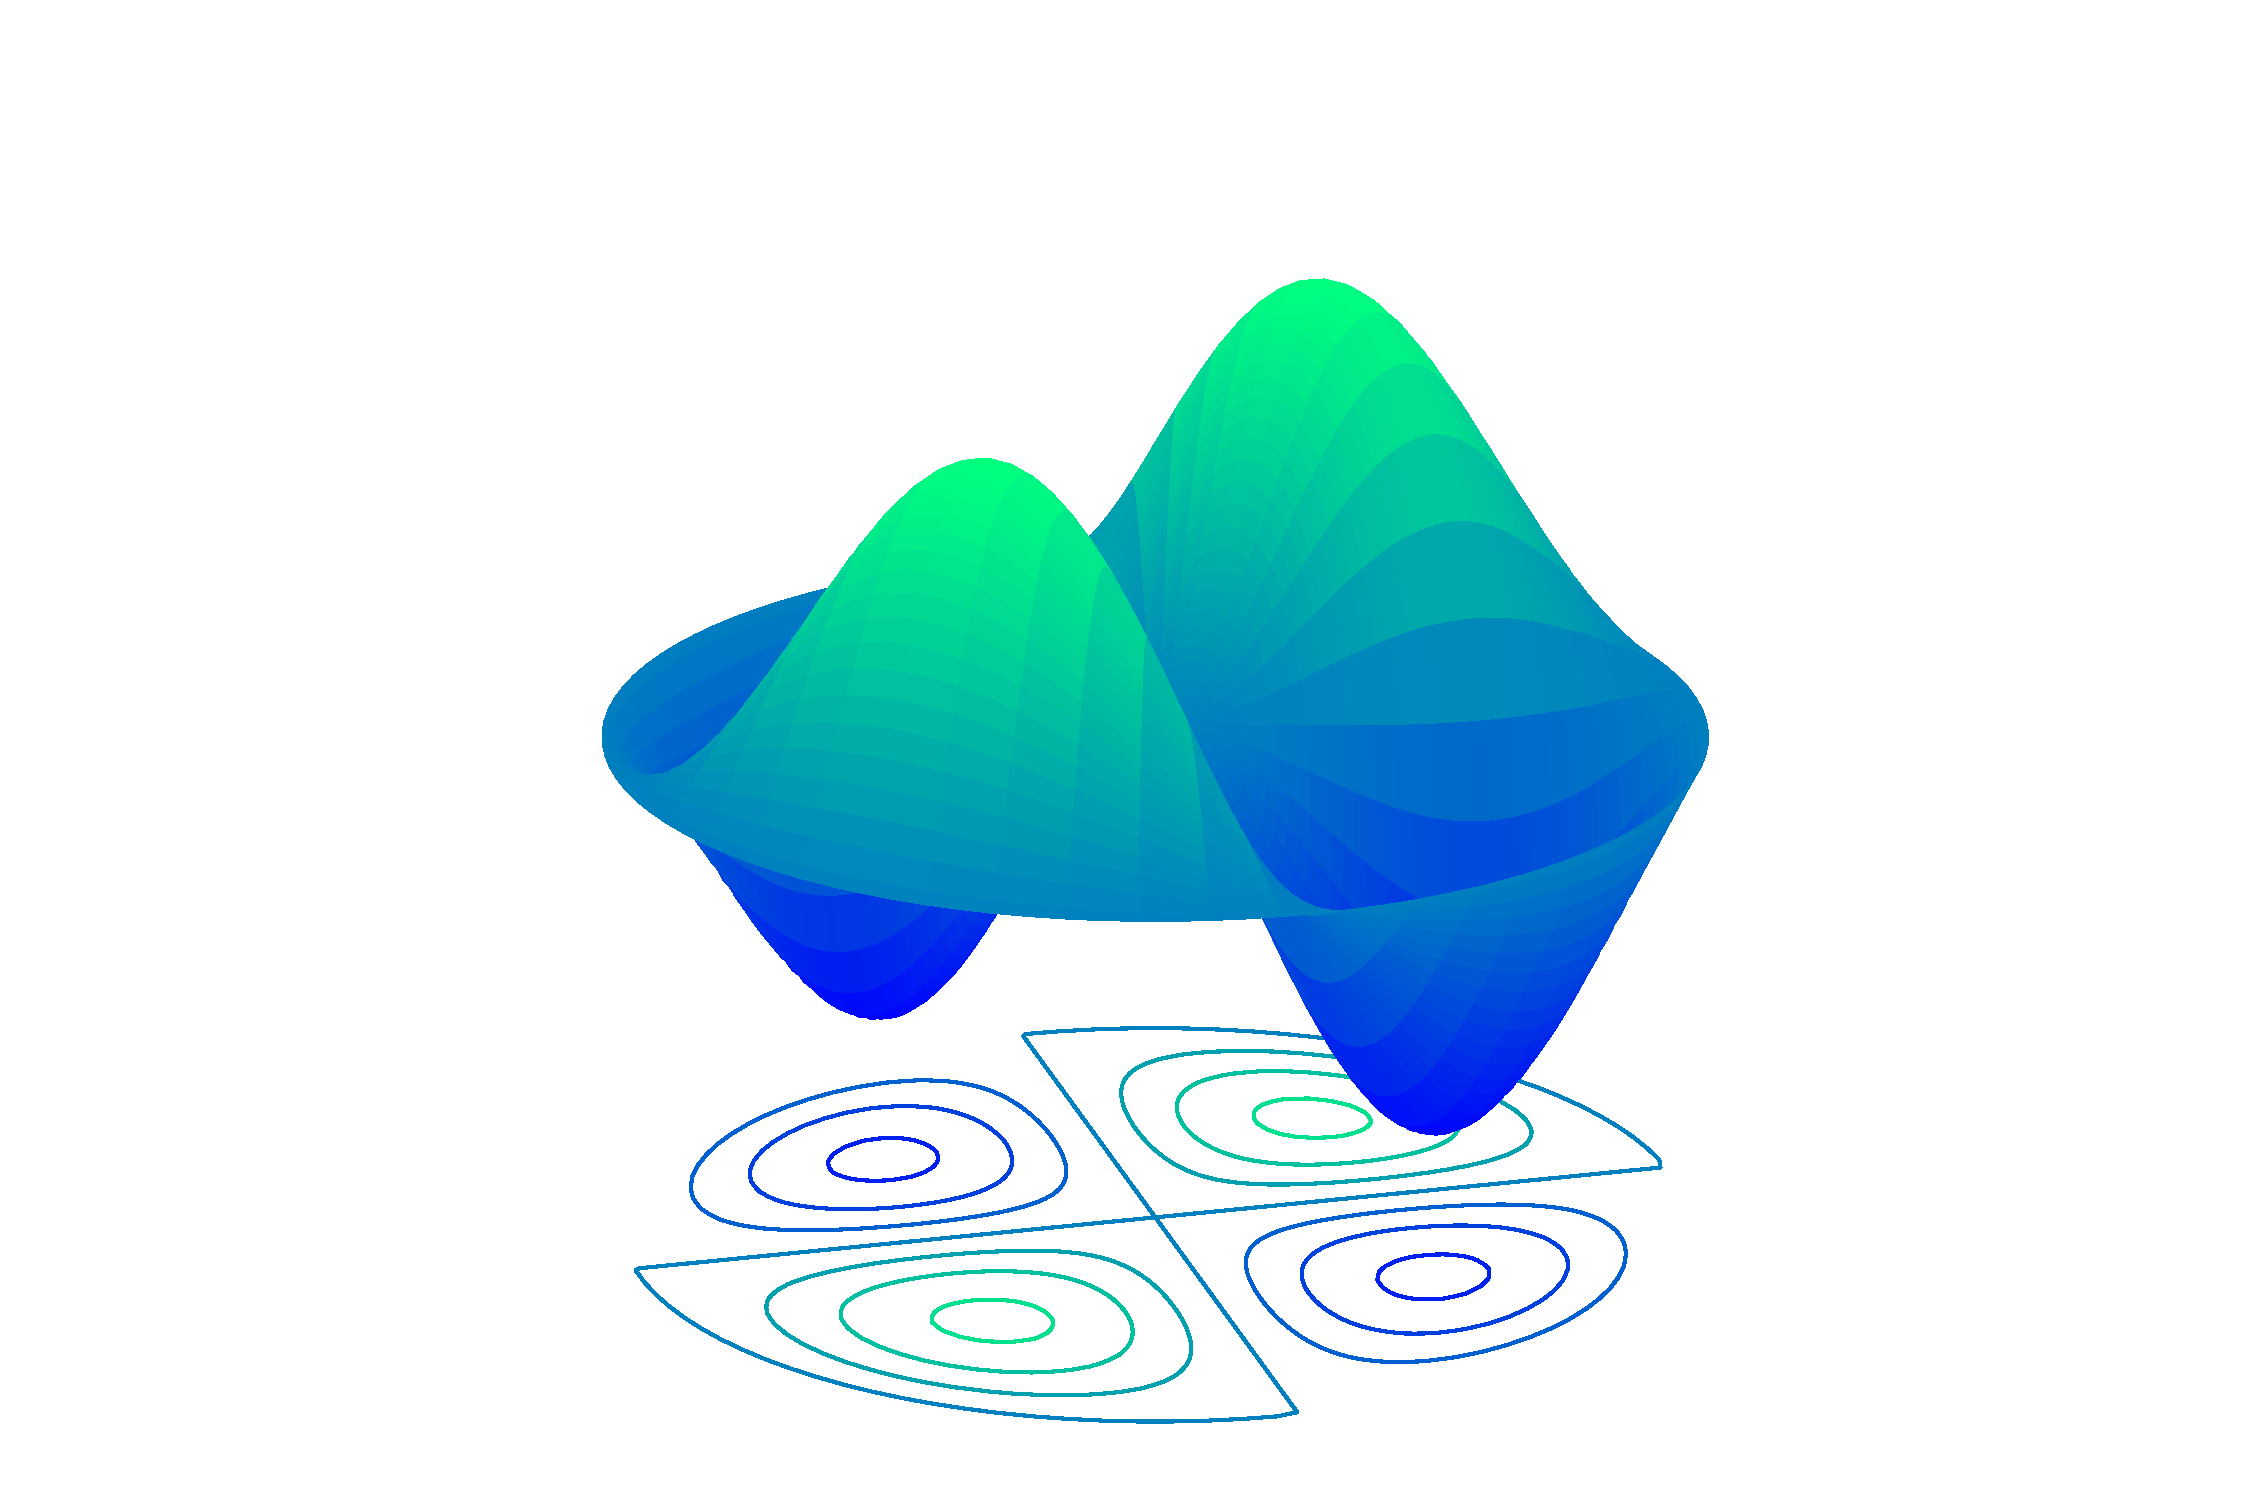
\includegraphics[scale=.16]{TCFE_4/modo_6.pdf}}
\end{minipage}%
\begin{minipage}{.5\linewidth}
\centering
\subfloat{\label{main:b}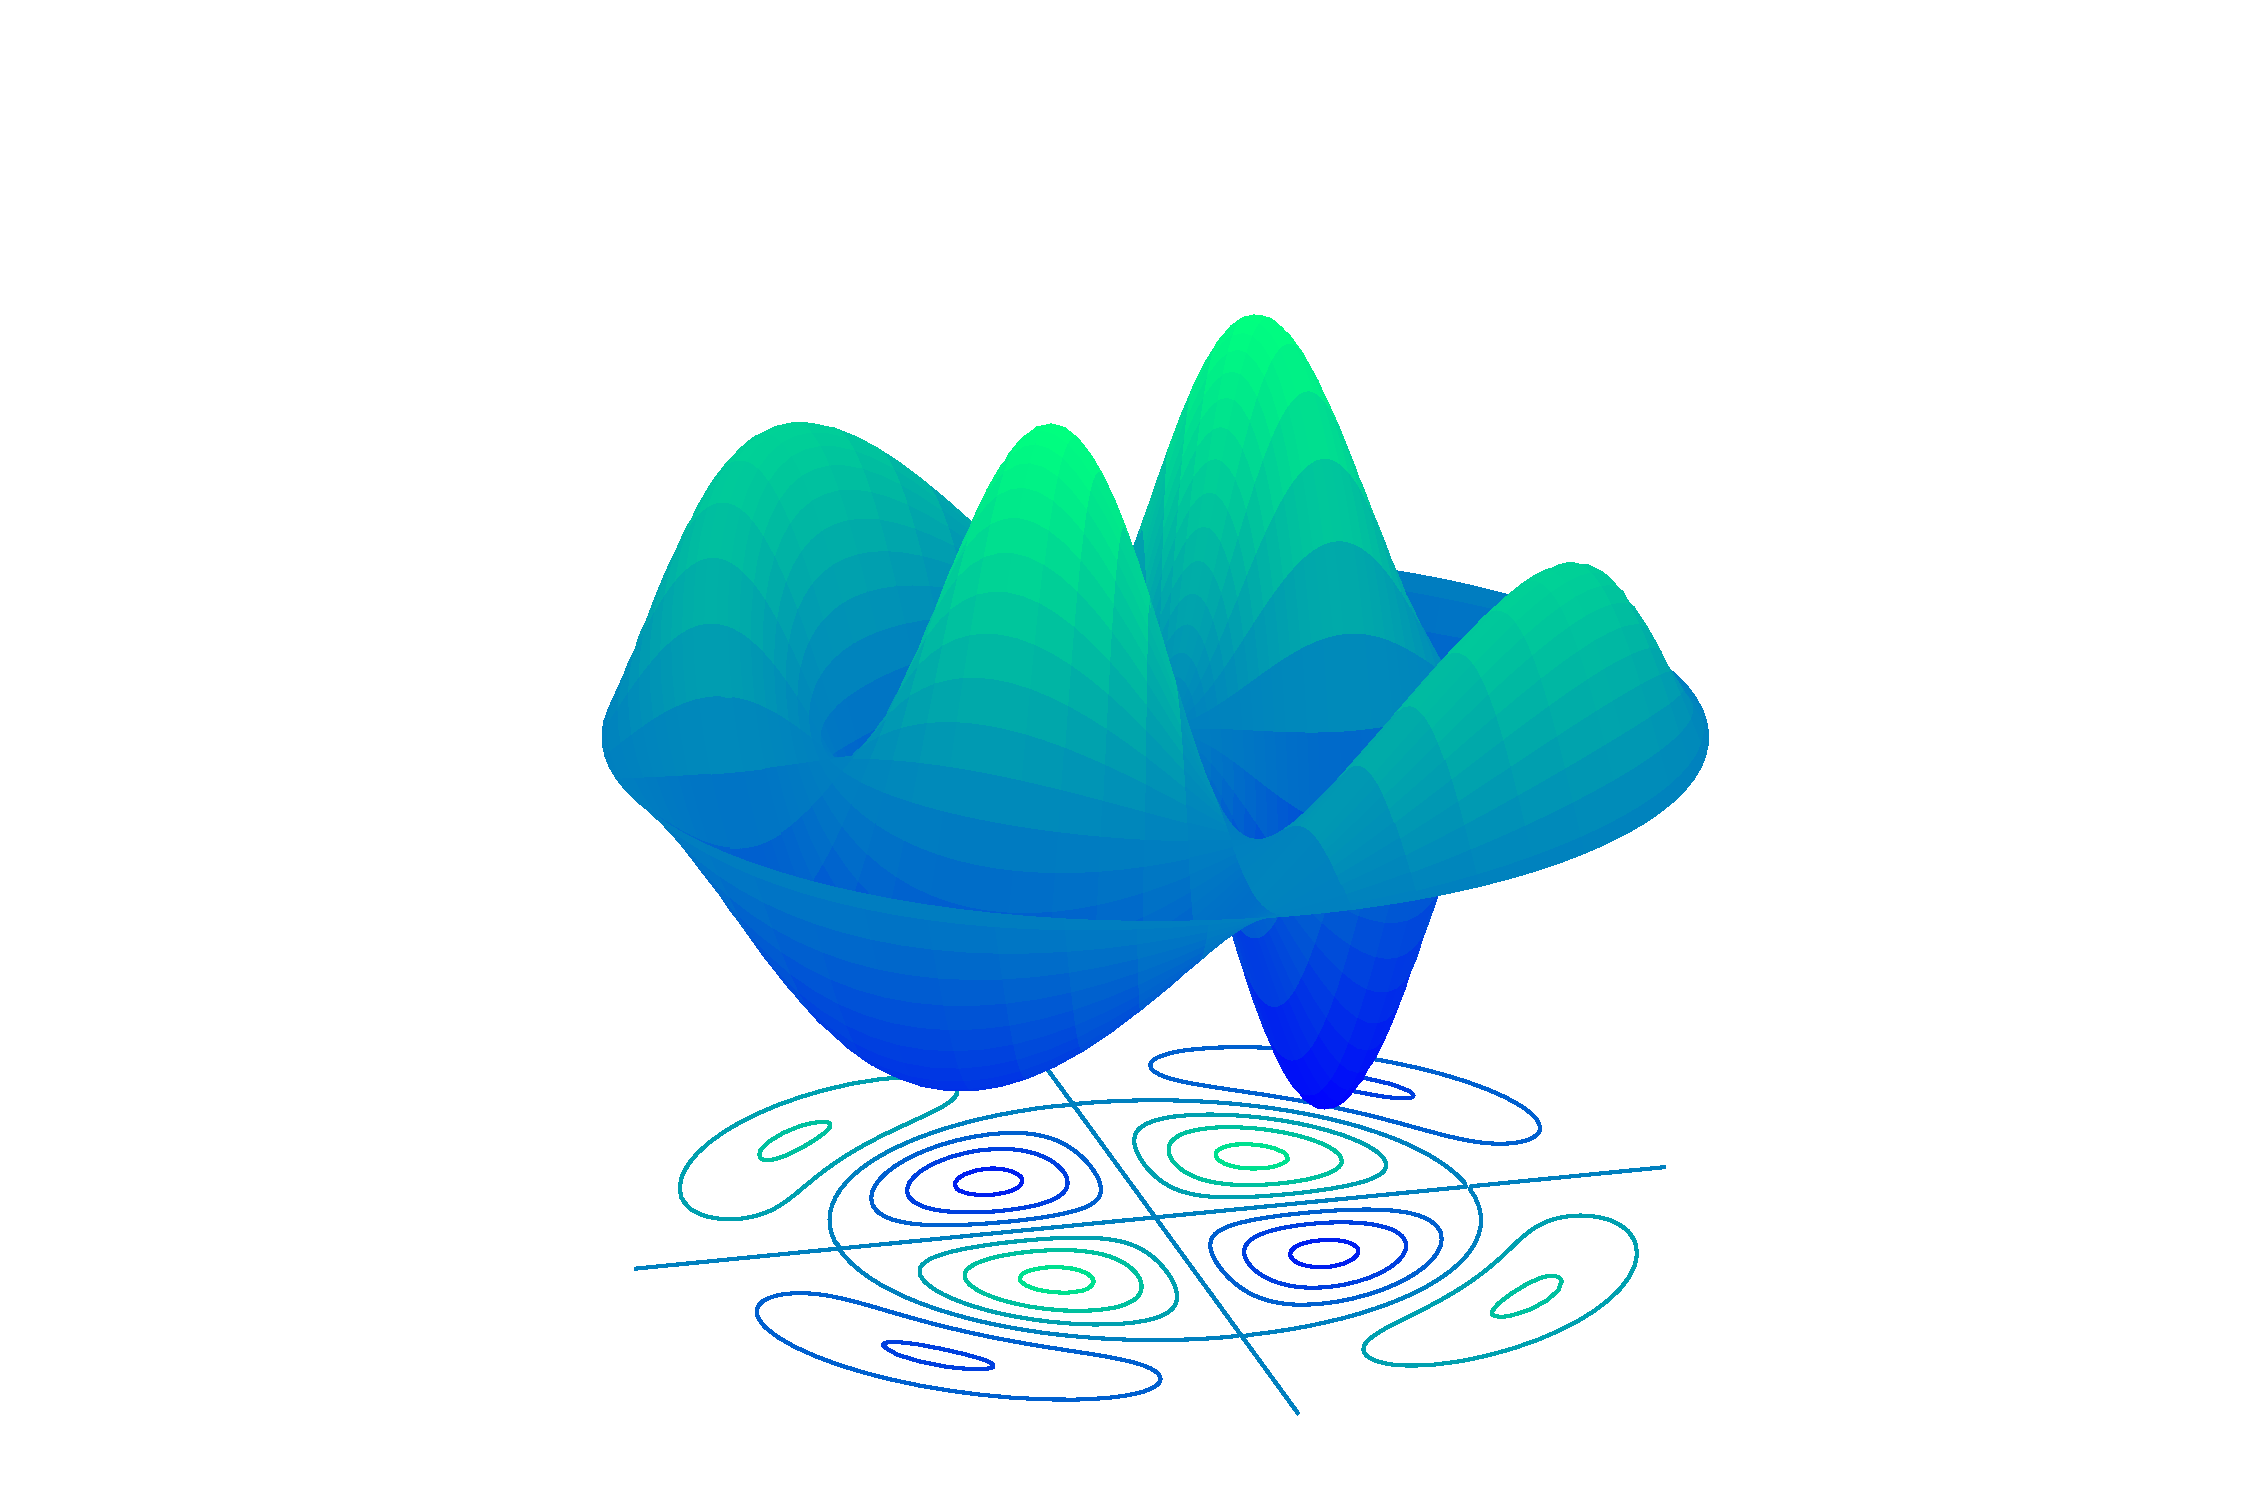
\includegraphics[scale=.16]{TCFE_4/modo_7.pdf}}
\end{minipage}\par\medskip
\centering
\subfloat{\label{main:c}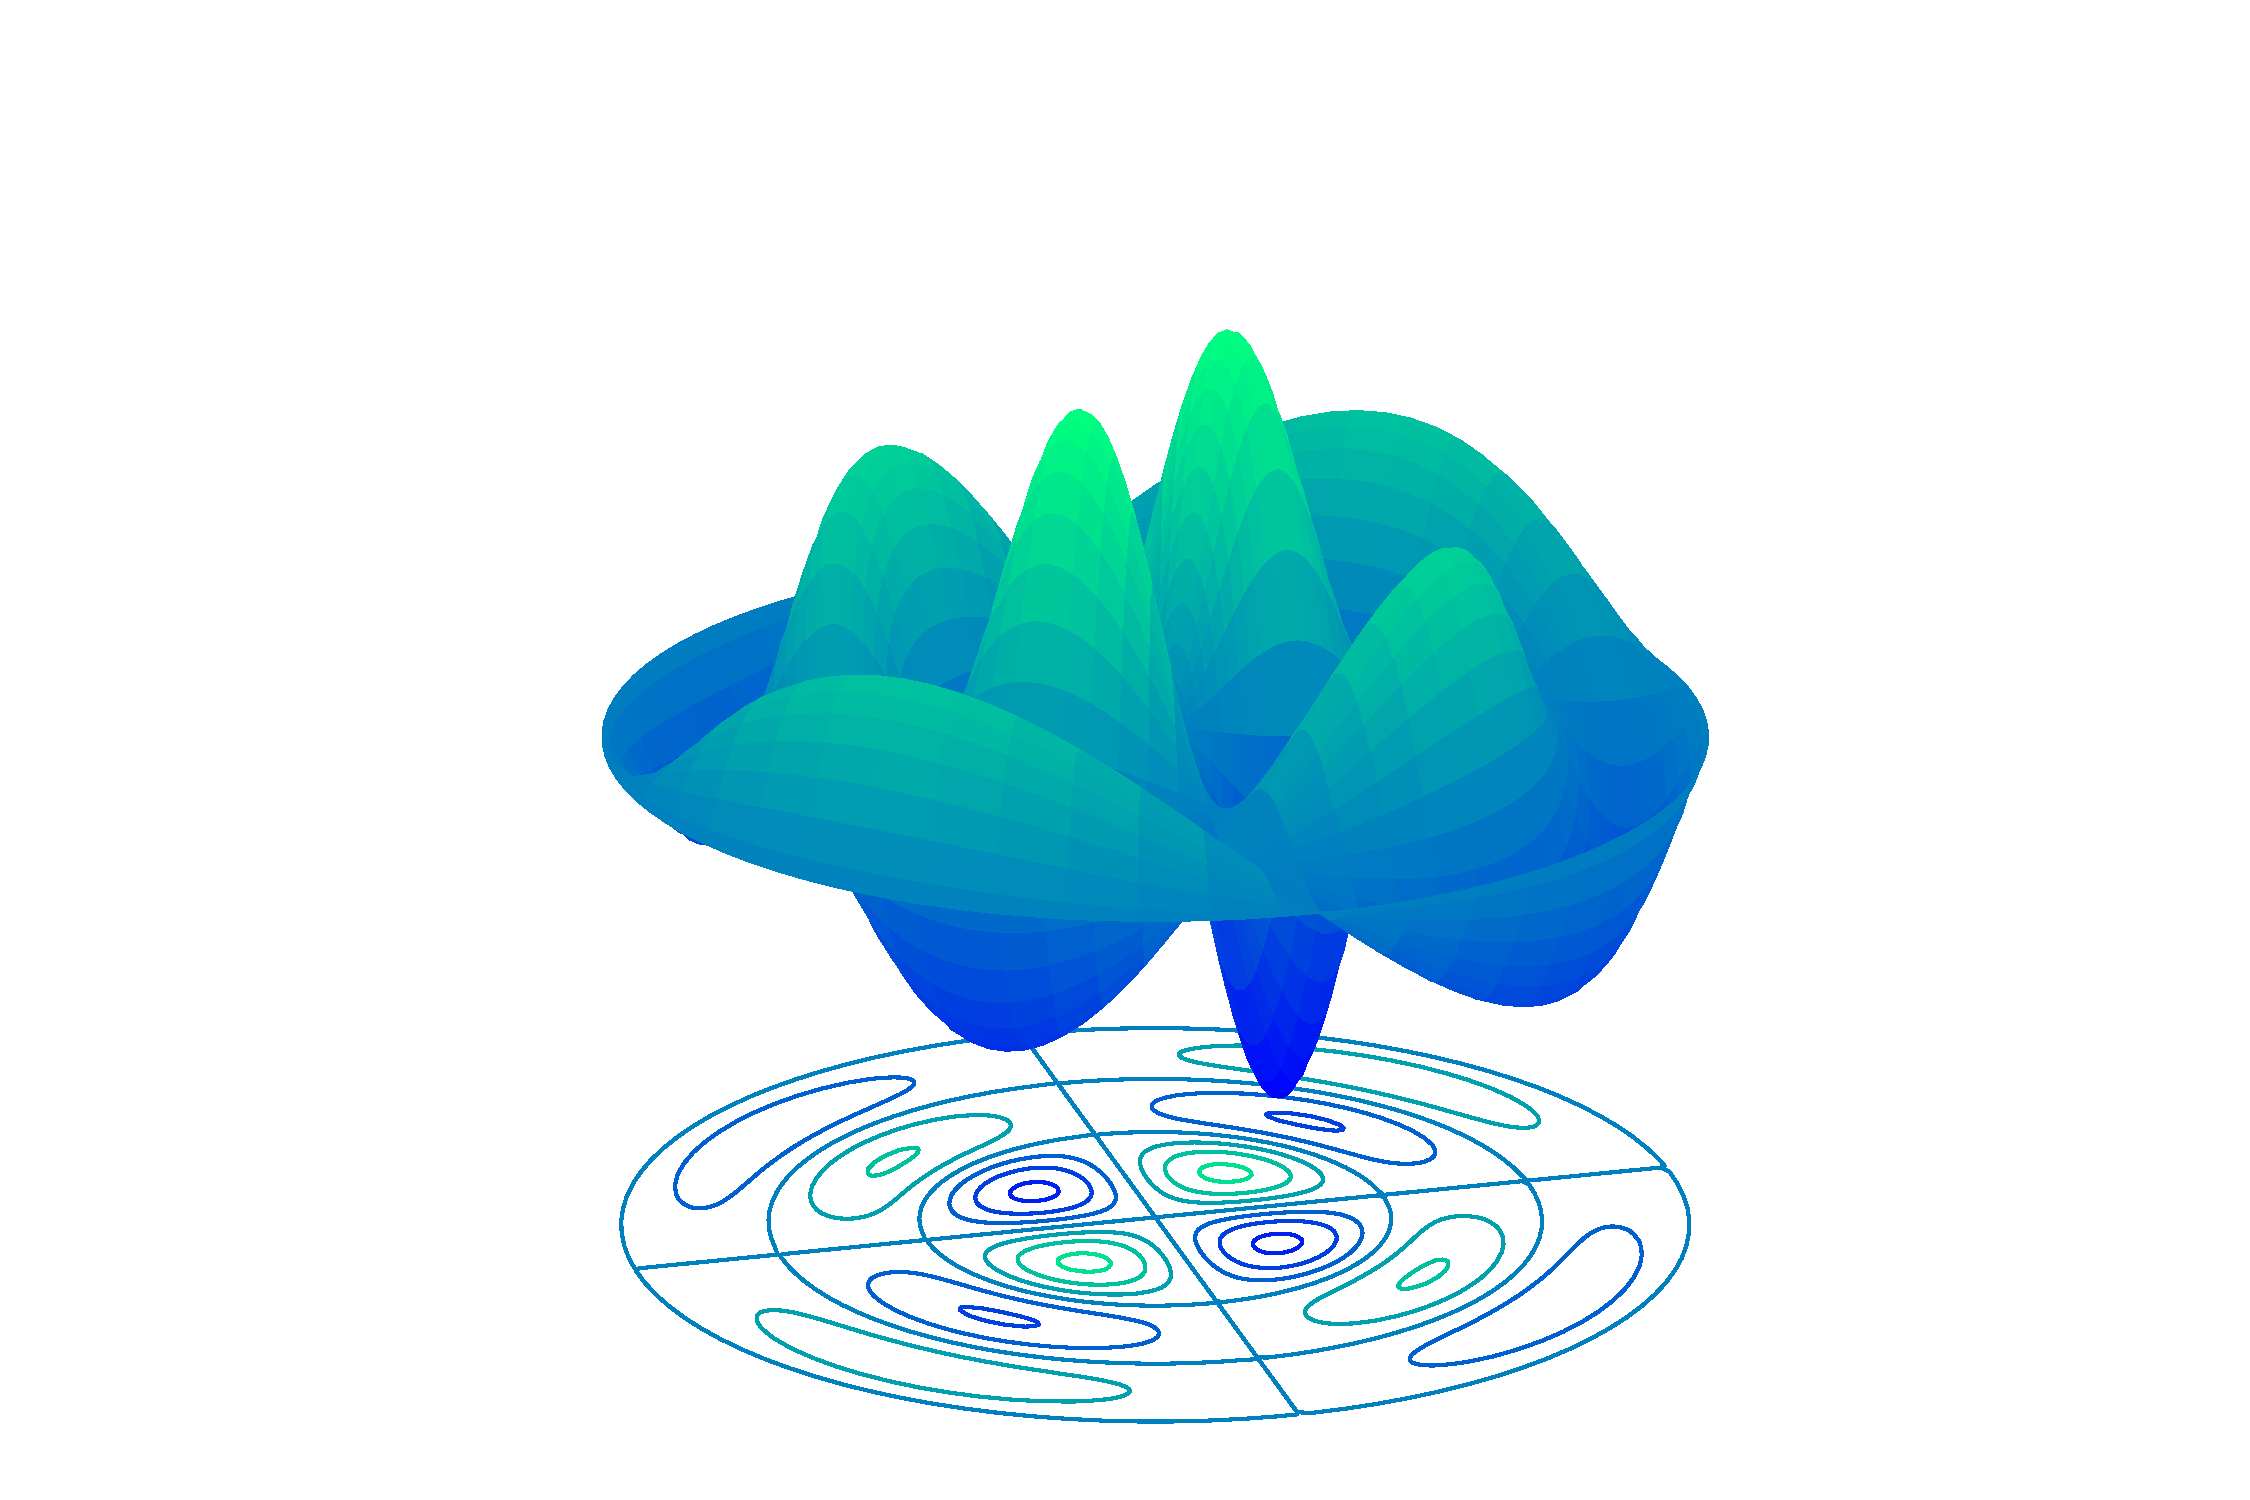
\includegraphics[scale=.16]{TCFE_4/modo_8.pdf}}

\caption{Apresentação gráfica dos resultados}
\label{fig:main}
\end{figure}

%----------------------------------------------------------------------------------------
\end{document}